%
% $XORP: xorp/docs/pim_testsuite/pim_testsuite.tex,v 1.2 2002/12/18 00:50:55 pavlin Exp $
%

\documentclass[11pt]{report}

%\usepackage[dvips]{changebar}

\usepackage{subfigure}
\usepackage{fullpage}
% \usepackage{setspace}         % XXX: enabling this breaks the compilation
\usepackage{times}
\usepackage{latexsym}
\usepackage{psfig}
\usepackage{graphicx}
\usepackage{xspace}
\usepackage{color}
%\usepackage[dvipdf]{graphics}
%\usepackage[dvips]{graphicx}

\definecolor{gray}{rgb}{0.5,0.5,0.5}
\newcommand{\etc}{\emph{etc.}\xspace}
\newcommand{\ie}{\emph{i.e.,}\xspace}
\newcommand{\eg}{\emph{e.g.,}\xspace}
%\newcommand{\comment}[1]{{\color{gray}[\textsf{#1}]}}
\newcommand{\comment}[1]{}

% Changebar stuff
% \newenvironment{colorcode}{\color{blue}}{}
% \renewcommand{\cbstart}{\begin{colorcode}}
% \renewcommand{\cbend}{\end{colorcode}}

% \pagestyle{empty}

\begin{document}

\title{XORP PIM-SM Test Suite \\
\vspace{1ex}
Version 0.1}
\author{ XORP Project                                   \\
         International Computer Science Institute       \\
         Berkeley, CA 94704, USA                        \\
         {\it feedback@xorp.org}
}
\date{December 11, 2002}

\maketitle

\thispagestyle{empty}


%%%%%%%%%%%%%%%%%%%%%%%%%%%%%%%%%%%%%%%%%%%%%%%%%%%%%%%%%%%%%%%%%%%%%%%
\newpage
\thispagestyle{empty}
{\huge \bf Modification History}
\vspace{4ex}

\begin{tabular}{lll}
Version 0.1 completed	& December 5, 2002 & \verb=draft-ietf-pim-sm-v2-new-05.{ps,tex}= \\
			&		   & \verb=draft-ietf-pim-sm-bsr-02.{ps,tex}=
\end{tabular}

%%%%%%%%%%%%%%%%%%%%%%%%%%%%%%%%%%%%%%%%%%%%%%%%%%%%%%%%%%%%%%%%%%%%%%%
\newpage
{\huge \bf Authors}
\vspace{4ex}

\begin{tabular}{lll}
Pavlin Radoslavov	& XORP Project, ICSI & pavlin@icsi.berkeley.edu
\end{tabular}

%%%%%%%%%%%%%%%%%%%%%%%%%%%%%%%%%%%%%%%%%%%%%%%%%%%%%%%%%%%%%%%%%%%%%%%
\tableofcontents
\listoftables
\listoffigures

%%%%%%%%%%%%%%%%%%%%%%%%%%%%%%%%%%%%%%%%%%%%%%%%%%%%%%%%%%%%%%%%%%%%%%%
\setcounter{chapter}{-1}
\chapter{Introduction}

%%%%%%%%%%%%%%%%%%%%%%%%%%%%%%%%%%%%%%%%%%%
\section{Overview}

TODO

This document describes a set of tests for evaluating Protocol Independent
Multicast - Sparse Mode implementation.

%%%%%%%%%%%%%%%%%%%%%%%%%%%%%%%%%%%%%%%%%%%
\section{Test Software}

TODO

%%%%%%%%%%%%%%%%%%%%%%%%%%%%%%%%%%%%%%%%%%%
\section{Acronyms}

Acronyms used in this Test Suite:

\begin{itemize}
  \item {\bf LAN}: {\bf L}ocal {\bf A}rea {\bf N}etwork
  \item {\bf M}: {\bf M}onitor or packet capturer
  \item {\bf MRT}: {\bf M}ulticast {\bf R}outing {\bf T}able
  \item {\bf MRE}: {\bf M}ulticast {\bf R}outing {\bf E}ntry
  \item {\bf MRIB}: {\bf M}ulticast {\bf R}outing {\bf I}nformation {\bf B}ase
  \item {\bf N}: {\bf N}etwork
  \item {\bf NBMA}: {\bf N}on-{\bf B}roadcast {\bf M}ulti-{\bf A}ccess
  \item {\bf RTE}: {\bf R}outing {\bf T}able {\bf E}ntry
  \item {\bf RUT}: {\bf R}outer {\bf U}nder {\bf T}est
  \item {\bf Rx}: {\bf R}eceiver
  \item {\bf S}: {\bf S}ource
  \item {\bf TN}: {\bf T}esting {\bf N}ode
  \item {\bf TR}: {\bf T}esting {\bf R}outer
\end{itemize}

When several entities of the same type are present in a test configuration, a
number is appended to the acronym to yield a label for each entity. For
example, if there were three testing routers in the test configuration, they
would be labeled TR1, TR2, TR3.

%%%%%%%%%%%%%%%%%%%%%%%%%%%%%%%%%%%%%%%%%%%
\section{Definitions}

TODO

%%%%%%%%%%%%%%%%%%%%%%%%%%%%%%%%%%%%%%%%%%%
\section{Timers and Default Values}
PIM-SMv2 defines several timers and default values. For the purpose of
testing, all configurable timers and values are set to their defaults, unless
otherwise noted in the test description. These defaults are given here for
reference, taken or calculated from the PIM-SM spec.

%
% PIM-SM spec values
%
\newcommand{\PimsmVersionDefault}{PIM-SMv2}	       % PIM_SM_version_default
\newcommand{\PimsmLanDelayDefault}{0.5 sec}		% LAN_delay_default
\newcommand{\PimsmTOverrideDefault}{2.5 sec}		% t_override_default
\newcommand{\PimsmHelloPeriod}{30 sec}			% Hello_Period
\newcommand{\PimsmTriggeredHelloDelay}{5 sec}		% Triggered_Hello_Delay
\newcommand{\PimsmDefaultHelloHoldtime}{105 sec}       % Default_Hello_Holdtime
\newcommand{\PimsmHelloHoldtime}{105 sec}		% Hello_Holdtime
\newcommand{\PimsmJPHoldTime}{210}			% J/P_HoldTime
\newcommand{\PimsmJPOverrideIntervalI}{3 sec}	     % J/P_Override_Interval(I)
\newcommand{\PimsmAssertOverrideInterval}{3 sec}     % Assert_Override_Interval
\newcommand{\PimsmAssertTime}{180 sec}			% Assert_Time
\newcommand{\PimsmTPeriodic}{60 sec}			% t_periodic
\newcommand{\PimsmTSuppressed}{rand(66, 84) sec}	% t_suppressed
\newcommand{\PimsmTOverride}{rand(0, 2.5) sec}		% t_override
\newcommand{\PimsmKeepalivePeriod}{210 sec}		% Keepalive_Period
\newcommand{\PimsmRPKeepalivePeriod}{185 sec}		% RP_Keepalive_Period
\newcommand{\PimsmRegisterSuppressionTime}{60 sec}  % Register_Suppression_Time
\newcommand{\PimsmRegisterProbeTime}{5 sec}		% Register_Probe_Time

%
% PIM-SM Bootstrap mechanism spec values
%
\newcommand{\PimsmBSPeriod}{60 sec}			% BS_Period
\newcommand{\PimsmBSTimeout}{130 sec}			% BS_Timeout
\newcommand{\PimsmRandOverride}{rand(0, 5.0) sec}	% rand_override
\newcommand{\PimsmCRPTimeout}{150 sec}			% C-RP_Timeout
\newcommand{\PimsmCRPAdvPeriod}{60 sec}			% C-RP-Adv_Period
\newcommand{\PimsmSZTimeout}{1500 sec}			% SZ_Timeout

\begin{itemize}

\item PIM-SM protocol spec:

\begin{tabular}{ll}
\verb=PIM_SM_version_default=	& 2		\\	% XXX: no such variable
\verb=LAN_delay_default=	& 0.5 sec	\\
\verb=t_override_default=	& 2.5 sec	\\
\verb=Hello_Period=		& 30 sec	\\
\verb=Triggered_Hello_Delay=	& 5 sec		\\
\verb=Default_Hello_Holdtime=	& 105 sec	\\
\verb=Hello_Holdtime=		& 105 sec	\\
\verb=J/P_HoldTime=		& 210 sec	\\
\verb=J/P_Override_Interval(I)=	& 3 sec		\\
\verb=Assert_Override_Interval=	& 3 sec		\\
\verb=Assert_Time=		& 180 sec	\\
\verb=t_periodic=		& 60 sec	\\
\verb=t_suppressed=		& rand(66, 84) sec \\
\verb=t_override=		& rand(0, 2.5) sec \\
\verb=Keepalive_Period=		& 210 sec	\\
\verb=RP_Keepalive_Period=	& 185 sec	\\
\verb=Register_Suppression_Time= & 60 sec	\\
\verb=Register_Probe_Time=	& 5 sec
\end{tabular}

\item Bootstrap mechanism spec:

\begin{tabular}{ll}
\verb=BS_Period=		& 60 sec	\\
\verb=BS_Timeout=		& 130 sec	\\
\verb=rand_override=		& rand(0, 5.0) sec \\
\verb=C-RP_Timeout=		& 150 sec	\\
\verb=C-RP-Adv_Period=		& 60 sec	\\
\verb=SZ_Timeout=		& 1500 sec
\end{tabular}

\end{itemize}

%%%%%%%%%%%%%%%%%%%%%%%%%%%%%%%%%%%%%%%%%%%
\section{Test Organization}

TODO

%%%%%%%%%%%%%%%%%%%%%%%%%%%%%%%%%%%%%%%%%%%
\section{References}

The following documents are referenced in this text:

\begin{itemize}

 \item RFC 2362 -- Protocol Independent Multicast-Sparse Mode (PIM-SM):
		  Protocol Specification

 \item \verb=draft-ietf-pim-sm-v2-new-05.{ps,tex}= -- Protocol Independent
		  Multicast - Sparse Mode (PIM-SM): Protocol Specification
		  (Revised)

 \item \verb=draft-ietf-pim-sm-bsr-02.{ps,tex}= -- Bootstrap Router (BSR)
		  Mechanism for PIM Sparse Mode

\end{itemize}


%%%%%%%%%%%%%%%%%%%%%%%%%%%%%%%%%%%%%%%%%%%
\section{Acknowledgments}
The format and notation in this test-suite is largely based on the format of
the IP Consortium Test Suite developed by the InterOperability Laboratory at
the University of New Hampshire.

%
% Test-suite specific setup
%
%\setlength{\parindent}{0ex}
\renewcommand{\chaptername}{Test Group}
%\newcommand{\para}[1]{\paragraph{\large #1}}
\newcommand{\para}[1]{\vspace{1ex}\noindent{\large\bf #1}}
%\newcommand{\subpara}[1]{\vspace{1ex}\noindent\emph{#1}\newline\noindent}
\newcommand{\subpara}[1]{\vspace{1ex}\noindent\emph{#1}}

%%%%%%%%%%%%%%%%%%%%%%%%%%%%%%%%%%%%%%%%%%%%%%%%%%%%%%%%%%%%%%%%%%%%%%%
\chapter{Interoperability}

\para{Scope:}
The following tests verify the general operation of a PIM-SM router and are
not specific to any single section of the specification.

\para{Overview:}
These tests have been designed to test the Interoperability of the RUT with
other PIM-SM capable devices. This test group focuses on testing
configurations of the network that could cause problems when deployed if the
RUT does not operate properly with the devices that it is connected to. The
tests in this group do not determine if a product conforms to the PIM-SM
standard but they are designed as interoperability tests. The test routers in
this section are complete implementation of PIM-SM.

Please note that in the case of interoperability tests, failure against any
other router does not necessarily indicate nonconformance. Rather, it
indicates that the two routers are unable to work ``properly'' together and
that further work should be done to isolate the cause of the failure.

%%%%%%%%%%%%%%%%%%%%%%%%%%%%%%%%%%%%%%%%%%%
\newpage
\section{Basic Interoperability}

\para{Purpose:}
To ensure that a router can interoperate with other PIM-SM
implementation in a multicast network.

\para{References:}
\begin{itemize}
  \item draft-ietf-pim-sm-v2-new-05 -- Section 4
\end{itemize}

\para{Discussion:}
PIM capable routers detect each other with PIM Hello
messages and exchange information for their routing tables through
PIM Join/Prune messages. For each multicast group there is a single PIM-SM
router that is the Rendezvous Point (RP) for that group. PIM-SM routers that
are connected to group members send PIM Join messages toward the RP to create
the group-specific shared tree. A PIM-SM router that is directly connected to
a multicast source, encapsulates the multicast data in PIM Register messages
which are unicast to the RP for that group. The RP decapsulates the
PIM Register messages and forwards them down the group-specific shared tree to
all receivers for that group.

\para{Test Setup:}
Connect the RUT, TR1, TN1, and TN2 according to
Figure~\ref{fig:basic_interoperability}.
Enable PIM-SM on both the RUT and TR1.

\begin{figure}[htbp]
  \begin{center}
    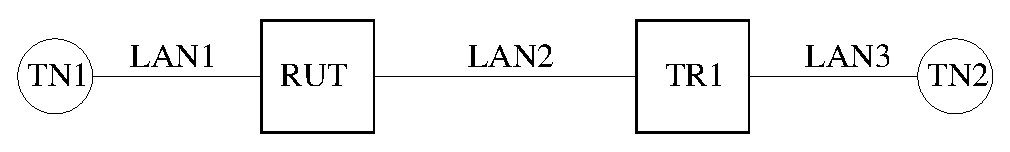
\includegraphics[scale=0.8]{figs/pim_test_1_1_basic_interoperability}
    \caption{Basic interoperability test setup}
    \label{fig:basic_interoperability}
  \end{center}
\end{figure}

\para{Procedure:}

\subpara{Part A: The RUT is the RP, TN1 is the receiver, and TN2 is the
sender.}

Configure both the RUT and TR1 such that the RUT is the RP for group
224.0.1.20. This configuration can be either manual, or implicit through the
Bootstrap mechanism. Configure TN1 and TN2 such that TN1 is the receiver, and
TN2 is the sender, both for group 224.0.1.20.

\begin{enumerate}

  \item Start both the RUT and TR1. If necessary, wait until the RP-set in the
        RUT and TR1 converges.

  \item Start the receiver and the sender.

  \item Observe the data packets received by the receiver.

\end{enumerate}

\subpara{Part B: TR1 is the RP, TN1 is the receiver, and TN2 is the sender.}

Configure both the RUT and TR1 such that TR1 is the RP for group
224.0.1.20. This configuration can be either manual, or implicit through the
Bootstrap mechanism. Configure TN1 and TN2 such that TN1 is the receiver, and
TN2 is the sender, both for group 224.0.1.20. The rest of the procedure is
same as in Part A.

\subpara{Part C: The RUT is the RP, TN2 is the receiver, and TN1 is the
sender.}

Configure both the RUT and TR1 such that the RUT is the RP for group
224.0.1.20. This configuration can be either manual, or implicit through the 
Bootstrap mechanism. Configure TN1 and TN2 such that TN2 is the receiver, and
TN1 is the sender, both for group 224.0.1.20. The rest of the procedure is
same as in Part A.

\subpara{Part D: TR1 is the RP, TN2 is the receiver, and TN1 is the sender.}

Configure both the RUT and TR1 such that TR1 is the RP for group
224.0.1.20. This configuration can be either manual, or implicit through the
Bootstrap mechanism. Configure TN1 and TN2 such that TN2 is the receiver, and
TN1 is the sender, both for group 224.0.1.20. The rest of the procedure is
same as in Part A.

\para{Observable Results:}
In all cases the data packets by the sender should be received by the
receiver.

In Part A, the data packets from TN2 should be encapsulated in PIM Registers
by TR1, unicast to the RUT (the RP), decapsulated by RUT, and then forwarded
(using native multicast) to TN1.
In Part B, the data packets from TN2 should be forwarded by TR1 to the RUT
(using native multicast, because TR1 does not need to encapsulate PIM Registers
to itself), and then forwarded to TN1.
In Part C, the data packets from TN1 should be forwarded (using native
multicast) by the RUT to TR1, and then to TN2.
In Part D, the data packets from TN1 should be encapsulated in PIM Registers
by the RUT, unicast to TN (the RP), decapsulated by TN, and then forwarded
(using native multicast) to TN2.

\para{Possible Problems:}
If the RP-set is empty, or is not same for
the RUT and TR1, no multicast packets will be received by the receiver.

%%%%%%%%%%%%%%%%%%%%%%%%%%%%%%%%%%%%%%%%%%%%%%%%%%%%%%%%%%%%%%%%%%%%%%%
\chapter{Designated Routers (DR) and Hello Messages}

\para{Scope:}
Test PIM router neighbor discovery, option exchange, and DR election.

\para{Overview:}
PIM Hello messages are send periodically on each
PIM-enabled interface. They are used to discover neighboring PIM routers,
to exchange various options, and to elect a Designated Router (DR) per LAN.
Hello messages are also used to provide a keep-alive function to detect a
neighbor loss.

%%%%%%%%%%%%%%%%%%%%%%%%%%%%%%%%%%%%%%%%%%%
\newpage
\section{Hello Transmission}

\para{Purpose:}
Verify that a router properly sends Hello messages.

\para{References:}
\begin{itemize}
  \item draft-ietf-pim-sm-v2-new-05 -- Section 4.3.1
\end{itemize}

\para{Discussion:}
Neighbor discovery of PIM capable routers is accomplished by sending Hello
messages to the ALL-PIM-ROUTERS multicast address (224.0.0.13 for IPv4,
and ``ff02::d'' for IPv6). These Hello messages must contain the following:
\begin{itemize}

  \item The IP TTL MUST be set to one.

  \item The Type field must be set to 0, this designates a PIM Hello message.

\end{itemize}

The router should transmit the Hello messages at an interval of
\verb=Hello_Period= ({\PimsmHelloPeriod}).

\para{Test Setup:}
Connect the RUT according to Figure~\ref{fig:hello_transmission}.
Enable PIM-SM on the RUT.

\begin{figure}[htbp]
  \begin{center}
    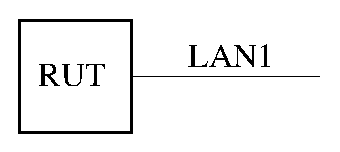
\includegraphics[scale=0.8]{figs/pim_test_2_1_hello_transmission}
    \caption{Hello transmission test setup}
    \label{fig:hello_transmission}
  \end{center}
\end{figure}

\para{Procedure:}
\begin{enumerate}

  \item Start the RUT.

  \item Observe the messages transmitted by the RUT.

\end{enumerate}

\para{Observable Results:}
\begin{itemize}

  \item The RUT should send properly formatted PIM Hello messages to the
        ALL-PIM-ROUTERS multicast address at \verb=Hello_Period=
        ({\PimsmHelloPeriod}) interval.

  \item The first Hello message only should be send after a random
        interval between 0 and \verb=Triggered_Hello_Delay=
        ({\PimsmTriggeredHelloDelay}).

  \item The PIM Hello messages should meet all the requirements in the
        discussion section.

\end{itemize}

\para{Possible Problems:}
None.

%%%%%%%%%%%%%%%%%%%%%%%%%%%%%%%%%%%%%%%%%%%
\newpage
\section{Two-Way Neighbor Adjacency}

\para{Purpose:}
Verify that a router accepts Hello messages and forms a two-way neighbor
adjacency.

\para{References:}
\begin{itemize}
  \item draft-ietf-pim-sm-v2-new-05 -- Section 4.3.1
\end{itemize}

\para{Discussion:}
Neighbor discovery of PIM capable routers is accomplished by sending Hello
messages to the ALL-PIM-ROUTERS address (224.0.0.13 for IPv4,
and ``ff02::d'' for IPv6). As a PIM router receives Hello messages from its
PIM neighbors, it records the neighbor addresses on each interface.

\para{Test Setup:}
Connect the RUT and TR1 according to
Figure~\ref{fig:two_way_neighbor_adjacency}.
Enable PIM-SM on both the RUT and TR1.

\begin{figure}[htbp]
  \begin{center}
    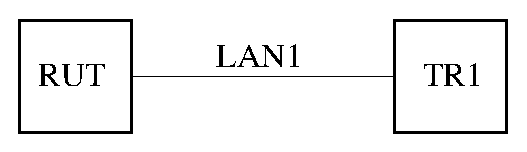
\includegraphics[scale=0.8]{figs/pim_test_2_2_two_way_neighbor_adjacency}
    \caption{Two-way neighbor adjacency test setup}
    \label{fig:two_way_neighbor_adjacency}
  \end{center}
\end{figure}

\para{Procedure:}

\subpara{Part A: Neighbor adjacency when there is network connectivity
failure.}

\begin{enumerate}

  \item Start the RUT.

  \item Observe the neighbor state information in the RUT for at least
        \verb=Triggered_Hello_Delay= ({\PimsmTriggeredHelloDelay}).

  \item Start TR1.

  \item Observe the neighbor state information in the RUT for at least
        \verb=Triggered_Hello_Delay= ({\PimsmTriggeredHelloDelay}).

  \item Disconnect TR1 from LAN1.

  \item Observe the neighbor state information in the RUT for at least
        \verb=Hello_Holdtime= ({\PimsmHelloHoldtime}).

\end{enumerate}

\subpara{Part B: Neighbor adjacency when a neighbor gracefully goes down.}

The procedure is same as in Part A, except that TR1 is gracefully shut-down
instead of disconnected from LAN1.

\subpara{Part C: Neighbor adjacency when the RUT is gracefully shut-down.}

\begin{enumerate}

  \item Start the RUT and TR1.

  \item Observe the neighbor state information in the RUT.

  \item Observe the messages transmitted by the RUT on LAN1.

  \item Gracefully shut-down the RUT.

\end{enumerate}

\para{Observable Results:}

\subpara{Part A:}

\begin{itemize}

  \item Before TR1 is started, the neighbor state information in the RUT should
        show no PIM neighbors:

\begin{verbatim}
Xorp> show pim neighbors 
Interface        DRpriority NeighborAddr    V Mode    Holdtime Timeout
\end{verbatim}

  \item After TR1 is started, and after up to \verb=Triggered_Hello_Delay=
        ({\PimsmTriggeredHelloDelay}), the neighbor state information in the
        RUT must contain TR1:

\begin{verbatim}
Xorp> show pim neighbors 
Interface        DRpriority NeighborAddr     V Mode    Holdtime Timeout
dc1                       1 10.2.0.2         2 Sparse       105     103
\end{verbatim}

  \item After TR1 is disconnected from LAN1, and after up to
        \verb=Hello_Holdtime= ({\PimsmHelloHoldtime}), the neighbor state
        information in the RUT should show no PIM neighbors:

\begin{verbatim}
Xorp> show pim neighbors 
Interface        DRpriority NeighborAddr     V Mode    Holdtime Timeout
\end{verbatim}

\end{itemize}

\subpara{Part B:}

The observed results should be same as in Part A, except that after TR1 is
gracefully shut-down, it would send a Hello message with zero \verb=HoldTime=.
After the RUT receives this Hello message, it should immediately timeout TR1,
instead of up to  \verb=Hello_Holdtime= ({\PimsmHelloHoldtime}).

\subpara{Part C:}

\begin{itemize}

  \item After TR1 is started, and after up to \verb=Triggered_Hello_Delay=
        ({\PimsmTriggeredHelloDelay}), the neighbor state information in the
        RUT must contain TR1:

\begin{verbatim}
Xorp> show pim neighbors 
Interface        DRpriority NeighborAddr     V Mode    Holdtime Timeout
dc1                       1 10.2.0.2         2 Sparse       105     103
\end{verbatim}

  \item Right after the RUT is gracefully shut-down, it should send
        a Hello message with zero \verb=HoldTime=.

\end{itemize}

\para{Possible Problems:}
None.

%%%%%%%%%%%%%%%%%%%%%%%%%%%%%%%%%%%%%%%%%%%
\newpage
\section{Hello Reception}

\para{Purpose:}
Verify that a router properly receives Hello messages.

\para{References:}
\begin{itemize}
  \item draft-ietf-pim-sm-v2-new-05 -- Sections 4.3.1, 4.10, and 4.10.2
\end{itemize}

\para{Discussion:}
Neighbor discovery of PIM capable routers is accomplished by sending Hello
messages to the ALL-PIM-ROUTERS address (224.0.0.13 for IPv4,
and ``ff02::d'' for IPv6). As a PIM router receives Hello messages from its
PIM neighbors, it records the neighbor addresses on each interface.
The checksum is 16-bit one's complement of the one's complement sum of the PIM
messages. The checksum MUST be validated on reception of the message.
The unused and reserved bits MUST be ignored upon reception.

\para{Test Setup:}
Connect the RUT and TR1 according to Figure~\ref{fig:hello_reception}.
Enable PIM-SM on both the RUT and TR1.

\begin{figure}[htbp]
  \begin{center}
    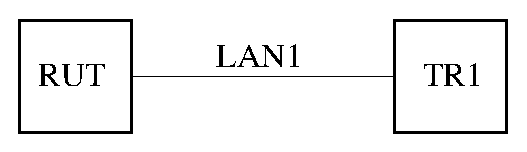
\includegraphics[scale=0.8]{figs/pim_test_2_3_hello_reception}
    \caption{Hello reception test setup}
    \label{fig:hello_reception}
  \end{center}
\end{figure}

\para{Procedure:}

\subpara{Part A: Reception of a PIM Hello message containing an invalid
checksum.}

\begin{enumerate}

  \item TR1 transmits a Hello message with an invalid checksum.

  \item Observe the neighbor state information in the RUT.

\end{enumerate}

\subpara{Part B: Reception of a PIM Hello message containing a Reserved field
of 0xFF.}

\begin{enumerate}

  \item TR1 transmits a Hello message containing a Reserved field of 0xFF.

  \item Observe the neighbor state information in the RUT.

\end{enumerate}

\subpara{Part C: Reception of a PIM Hello message containing a Version field
of 0xF.}

\begin{enumerate}

  \item TR1 transmits a Hello message containing a Version field of 0xF.

  \item Observe the neighbor state information in the RUT.

\end{enumerate}

\subpara{Part D: Reception of a PIM message containing an unrecognized
Type field of 0xF.}

\begin{enumerate}

  \item TR1 transmits a PIM message containing a Type field of 0xF.

  \item Observe the warning log messages in the RUT.

\end{enumerate}

\para{Observable Results:}
\begin{itemize}

  \item In Part A, the Hello messages with invalid checksum should be ignored,
        and the neighbor state information in the RUT should show no PIM
        neighbors:

\begin{verbatim}
Xorp> show pim neighbors 
Interface        DRpriority NeighborAddr     V Mode    Holdtime Timeout
\end{verbatim}


  \item In Part B, after TR1 is started, and after up to
        \verb=Triggered_Hello_Delay=
        ({\PimsmTriggeredHelloDelay}), the neighbor state information in the
        RUT must contain TR1:

\begin{verbatim}
Xorp> show pim neighbors 
Interface        DRpriority NeighborAddr     V Mode    Holdtime Timeout
dc1                       1 10.2.0.2         2 Sparse       105     103
\end{verbatim}

  \item In Part C, after TR1 is started, and after up to
        \verb=Triggered_Hello_Delay=
        ({\PimsmTriggeredHelloDelay}), the neighbor state information in the
        RUT must contain TR1 with protocol version of 15 (0xF).

\begin{verbatim}
Xorp> show pim neighbors 
Interface        DRpriority NeighborAddr     V Mode    Holdtime Timeout
dc2                       1 10.3.0.1        15 Sparse       105     103
\end{verbatim}

  \item In Part D, after TR1 is started and after it sends PIM messages
        containing a Type field of 0xF, the RUT should log the messages with
        this unrecognized Type field:

\begin{verbatim}
[ 2002/08/17 22:45:20 WARNING test_pim.rut PIM ] RX PIM_type_unknown from
10.3.0.2 to 224.0.0.13: message type (15) is unknown
\end{verbatim}

\end{itemize}

\para{Possible Problems:}
\begin{itemize}

  \item Earlier protocol specification (RFC 2117), have ``Addr length''
        field in place of the ``Reserved'' field. Therefore, the test in Part
        B may not be appropriate for such implementations.

  \item At the moment of writing, the lastest
        PIM-SM spec does not describe the behavior if a PIM message is
        received with protocol version that is larger than the implemented
        one.
        (TODO: if the spec later is modified to include that behavior,
        remove this bullet).
        Hence, in Part C, it is possible that an implementation may
        silently ignore all messages with protocol version larger than
        \verb=PIM_SM_version_default= ({\PimsmVersionDefault}).
        As a result, the RUT will not see TR1 as a neighbor.

  \item In Part D, the RUT may not log events such as receiving of a message
        with unrecognized Type field, because the logging is not described
        in the spec.

\end{itemize}

%%%%%%%%%%%%%%%%%%%%%%%%%%%%%%%%%%%%%%%%%%%
\newpage
\section{Holdtime Option}

\para{Purpose:}
Verify that a router properly sends and receives Hello messages with Holdtime
option.

\para{References:}
\begin{itemize}
  \item draft-ietf-pim-sm-v2-new-05 -- Sections 4.3.1 and 4.10.2
\end{itemize}

\para{Discussion:}
PIM capable routers periodically send Hello messages
messages to the ALL-PIM-ROUTERS address (224.0.0.13 for IPv4,
and ``ff02::d'' for IPv6). If a PIM router does not receive a Hello message
from a neighbor for some amount of time, it is assumed that the neighbor (or
the connectivity to it) is not operational, therefore the neighbor is
timed-out. A Hello message may contain a Holdtime option that specifies the
amount of time (in seconds) a router must keep the neighbor reachable.
If a Hello message does not contain a Holdtime option, the default value
of \verb=Default_Hello_Holdtime= ({\PimsmDefaultHelloHoldtime})
is assumed. If a Hello message contains a Holdtime option with value of
0xFFFF, then only one Hello message should be sent, and the router-recipient
of the message should not time-out the router-originator.

\para{Test Setup:}
Connect the RUT and TR1 according to Figure~\ref{fig:holdtime_option}.
Enable PIM-SM on both the RUT and TR1.

\begin{figure}[htbp]
  \begin{center}
    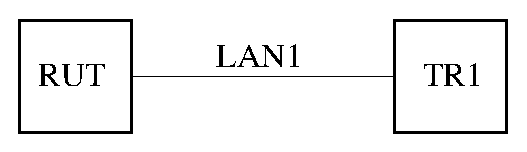
\includegraphics[scale=0.8]{figs/pim_test_2_4_holdtime_option}
    \caption{Holdtime option test setup}
    \label{fig:holdtime_option}
  \end{center}
\end{figure}

\para{Procedure:}

\subpara{Part A: Transmission of a PIM Hello message containing a Holdtime
option.}

\begin{enumerate}

  \item Start the RUT.

  \item Observe the messages transmitted by the RUT for at least
        \verb=Triggered_Hello_Delay= + 3 * \verb=Hello_Holdtime=
        (\ie ({\PimsmTriggeredHelloDelay}) + 3 * ({\PimsmHelloHoldtime})).

  \item Stop the RUT.

  \item Observe the messages transmitted by the RUT for at least
        \verb=Triggered_Hello_Delay= + 3 * \verb=Hello_Holdtime=
        (\ie ({\PimsmTriggeredHelloDelay}) + 3 * ({\PimsmHelloHoldtime})).

  \item Change the configuration value of \verb=Hello_Holdtime= and repeat.

\end{enumerate}

\subpara{Part B: Transmission of a PIM Hello message containing a Holdtime
option with value of 0xFFFF.}

The procedure is same as in Part A, except that the RUT is configured with
Holdtime option value of 0xFFFF. Note that the amount of time to observe the
transmitted messages should be same as in Part A.

\subpara{Part C: Reception of a PIM Hello message containing a Holdtime
option.}

\begin{enumerate}

  \item Start the RUT.

  \item Observe the neighbor state information in the RUT for at least
        \verb=Triggered_Hello_Delay= ({\PimsmTriggeredHelloDelay}).

  \item Configure TR1 such that its Hello messages would contain a Holdtime
        option with the default value of \verb=Hello_Holdtime=
        ({\PimsmHelloHoldtime}).

  \item Start TR1.

  \item Observe the neighbor state information in the RUT for at least
        \verb=Triggered_Hello_Delay= ({\PimsmTriggeredHelloDelay}).

  \item Stop TR1.

  \item Observe the neighbor state information in the RUT for at least
        \verb=Hello_Holdtime= ({\PimsmHelloHoldtime}).

  \item Change the configuration value of \verb=Hello_Holdtime= in TR1 and
        repeat.

\end{enumerate}

\subpara{Part D: Reception of a PIM Hello message containing a Holdtime option
with value of 0xFFFF.}

The procedure is same as in Part C, except that in Step 3 the Hello message
originated by TR1 must be configured contain a Holdtime option with value of
0xFFFF.

\subpara{Part E: Reception of a PIM Hello message that does not contain a
Holdtime option.}

The procedure is same as in Part C, except that in Step 3 the the Hello message
originated by TR1 must be configured to exclude the Holdtime option.

\para{Observable Results:}

\subpara{Part A:}

\begin{itemize}

  \item After the RUT is started, the first Hello message should be
        transmitted no later than \verb=Triggered_Hello_Delay=
        ({\PimsmTriggeredHelloDelay}).

  \item After the first Hello message, there should be one Hello message
        transmitted each \verb=Hello_Period= ({\PimsmHelloPeriod}). Each Hello
        message should contain a Holdtime option with default value of
        \verb=Hello_Holdtime= ({\PimsmHelloHoldtime}).

  \item Right after the RUT is stopped, there should be
        a Hello message transmitted with Holdtime option value of 0.

  \item After the Hello message with Holdtime option value of 0,
        no other Hello messages should be transmitted.

  \item The results of repeating the test with different value of
        \verb=Hello_Holdtime= should be similar, except that the
        Hello messages should be transmitted every 1/3th of
        the new \verb=Hello_Holdtime=, and the Holdtime Option value
        in the Hello messages should be the new \verb=Hello_Holdtime=.

\end{itemize}

\subpara{Part B:}

\begin{itemize}

  \item After the RUT is started, the first Hello message should be
        transmitted no later than \verb=Triggered_Hello_Delay=
        ({\PimsmTriggeredHelloDelay}). This message should contain
        a Holdtime option with value of 0xFFFF.

  \item After the first Hello message, there should be no one Hello messages
        transmitted before the RUT is stopped.

  \item Right after the RUT is stopped, there should be
        a Hello message transmitted with Holdtime option value of 0.

  \item After the Hello message with Holdtime option value of 0,
        no other Hello messages should be transmitted.

\end{itemize}

\subpara{Part C:}

\begin{itemize}

  \item Before TR1 is started, the neighbor state information in the RUT
  should show no PIM neighbors:

\begin{verbatim}
Xorp> show pim neighbors
Interface        DRpriority NeighborAddr    V Mode    Holdtime Timeout
\end{verbatim}

  \item After TR1 is started, and after up to \verb=Triggered_Hello_Delay=
        ({\PimsmTriggeredHelloDelay}), the neighbor state information in the
        RUT must contain TR1. The Holdtime information about TR1 must match
        the Holdtime value in the Hello messages by TR1:

\begin{verbatim}
Xorp> show pim neighbors
Interface        DRpriority NeighborAddr     V Mode    Holdtime Timeout
dc1                       1 10.2.0.2         2 Sparse       105     103
\end{verbatim}

  \item After TR1 is stopped, and after it sends a Hello message with Holdtime
        option value of 0, the RUT must immediately expire it.
        The neighbor state information in the RUT should show no PIM
        neighbors:

\begin{verbatim}
Xorp> show pim neighbors
Interface        DRpriority NeighborAddr     V Mode    Holdtime Timeout
\end{verbatim}

  \item The results of repeating the test with different value of
        \verb=Hello_Holdtime= should be similar, except that the
        Holdtime value in the state information in the RUT about TR1 should
        match the chosen value of the \verb=Hello_Holdtime=.

\end{itemize}

\subpara{Part D:}

The observed results should be same as in Part C, except that
after the first Hello message from TR1 is received, the neighbor state
information in the RUT must show that the TR1 would never be expired:

\begin{verbatim}
Xorp> show pim neighbors 
Interface        DRpriority NeighborAddr     V Mode    Holdtime Timeout
dc1                       1 10.3.0.2         2 Sparse     65535    None
\end{verbatim}

\subpara{Part E:}

The observed results should be same as in Part C, except that
the RUT assumes that the Holdtime value about TR1 is always equal to the
default value of \verb=Hello_Holdtime= ({\PimsmHelloHoldtime}).

\para{Possible Problems:}
None.

%%%%%%%%%%%%%%%%%%%%%%%%%%%%%%%%%%%%%%%%%%%
\newpage
\section{DR Priority Option}

\para{Purpose:}
Verify that a router properly sends and receives Hello messages with DR
Priority option.

\para{References:}
\begin{itemize}
  \item draft-ietf-pim-sm-v2-new-05 -- Sections 4.3.1, 4.3.2, and 4.10.2
\end{itemize}

\para{Discussion:}
One of the PIM routers on each LAN, the Designated Router (DR), needs to act
on behalf of the rest of the routers and directly connected hosts with respect
to the PIM protocol. The DR election considers the DR priority of each
PIM router and its IP address: numerically larger DR priority is always
better, with a numerically larger IP address used as a tie-break. Each PIM
router includes its DR priority in the DR Priority option of the Hello
messages it originates. If there is at least one PIM router on a LAN that does
not include the DR Priority option in its Hello messages, then the DR election
process considers only the IP addresses of the routers.

\para{Test Setup:}
Connect the RUT and TR1 according to Figure~\ref{fig:dr_priority_option}.
Enable PIM-SM on both the RUT and TR1.

\begin{figure}[htbp]
  \begin{center}
    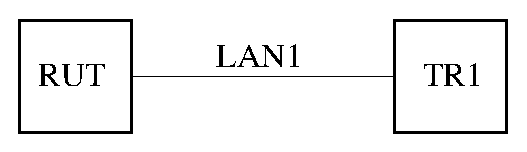
\includegraphics[scale=0.8]{figs/pim_test_2_5_dr_priority_option}
    \caption{DR priority option test setup}
    \label{fig:dr_priority_option}
  \end{center}
\end{figure}

\para{Procedure:}

\subpara{Part A: The RUT has a numerically larger IP address than TR1.}

\begin{enumerate}

  \item Start the RUT with default DR priority of 1, and
        observe the DR state information in the RUT.

  \item Start TR1 with default DR priority of 1, and
        observe the DR state information in the RUT.

  \item Change the DR priority of TR1 to 2, and
        observe the DR state information in the RUT.

  \item Change the DR priority of TR1 to 0, and
        observe the DR state information in the RUT.

  \item Change the DR priority of TR1 to 1, and
        observe the DR state information in the RUT.

  \item Change the DR priority of the RUT to 2, and
        observe the DR state information in the RUT.

  \item Change the DR priority of the RUT to 0, and
        observe the DR state information in the RUT.

  \item Change the DR priority of the RUT to 1, and
        observe the DR state information in the RUT.

\end{enumerate}

\subpara{Part B: The RUT has a numerically smaller IP address than TR1.}

The procedure is same as in Part A, except that TR1 has a numerically smaller
IP address than TR1.

\para{Observable Results:}

\subpara{Part A:}

\begin{enumerate}

  \item After the RUT is started with default DR priority of 1, it should
        be the DR for LAN1:

\begin{verbatim}
Xorp> show pim interface dc2
Interface       State    Mode    V PIMstate  Priority DRaddr      Neighbors
dc2             UP       Sparse  2 DR               1 10.2.0.2            0
\end{verbatim}

  \item After TR1 is started with default DR priority of 1, the RUT should be
        still the DR for LAN1:

\begin{verbatim}
Xorp> show pim interface dc2
Interface       State    Mode    V PIMstate  Priority DRaddr      Neighbors
dc2             UP       Sparse  2 DR               1 10.2.0.2            1
\end{verbatim}

  \item After the DR priority of TR1 is increased to 2, TR1 should become the
  DR for LAN1. The DR state information in the RUT should show that the RUT is
  not the DR anymore:

\begin{verbatim}
Xorp> show pim interface dc2
Interface       State    Mode    V PIMstate  Priority DRaddr      Neighbors
dc2             UP       Sparse  2 NotDR            1 10.2.0.1            1
\end{verbatim}

  \item After the DR priority of TR1 is decreased to 0, the RUT should become
        the DR for LAN1:

\begin{verbatim}
Xorp> show pim interface dc2
Interface       State    Mode    V PIMstate  Priority DRaddr      Neighbors
dc2             UP       Sparse  2 DR               1 10.2.0.2            1
\end{verbatim}

  \item After the DR priority of TR1 is increased to 1, the RUT should
        continue to be the DR for LAN1: 

\begin{verbatim}
Xorp> show pim interface dc2
Interface       State    Mode    V PIMstate  Priority DRaddr      Neighbors
dc2             UP       Sparse  2 DR               1 10.2.0.2            1
\end{verbatim}

  \item After the DR priority of the RUT is increased to 2, the RUT should
        continue to be the DR for LAN1:

\begin{verbatim}
Xorp> show pim interface dc2
Interface       State    Mode    V PIMstate  Priority DRaddr     Neighbors
dc2             UP       Sparse  2 DR               2 10.2.0.2           1
\end{verbatim}

  \item After the DR priority of the RUT is decreased to 0, TR1 should become
        the DR for LAN1. The DR state information in the RUT should show that
        the RUT is not the DR anymore:

\begin{verbatim}
Xorp> show pim interface dc2
Interface       State    Mode    V PIMstate  Priority DRaddr     Neighbors
dc2             UP       Sparse  2 NotDR            0 10.2.0.1           1
\end{verbatim}

  \item After the DR priority of the RUT is increased to 1, the RUT should
        become the DR for LAN1:

\begin{verbatim}
Xorp> show pim interface dc2
Interface       State    Mode    V PIMstate  Priority DRaddr      Neighbors
dc2             UP       Sparse  2 DR               1 10.2.0.2            1
\end{verbatim}

\end{enumerate}

\subpara{Part B:}

\begin{enumerate}

  \item After the RUT is started with default DR priority of 1, it should
        be the DR for LAN1:

\begin{verbatim}
Xorp> show pim interface dc2
Interface       State    Mode    V PIMstate  Priority DRaddr      Neighbors
dc2             UP       Sparse  2 DR               1 10.2.0.2            0
\end{verbatim}

  \item After TR1 is started with default DR priority of 1, it should become
        the DR for LAN1. The DR state information in the RUT should show that
        the RUT is not the DR anymore:

\begin{verbatim}
Xorp> show pim interface dc2
Interface       State    Mode    V PIMstate  Priority DRaddr      Neighbors
dc2             UP       Sparse  2 NotDR            1 10.2.0.3            1
\end{verbatim}

  \item After the DR priority of TR1 is increased to 2, TR1 should continue to
        be the DR for LAN1. The DR state information in the RUT should show
        that the RUT is not the DR:

\begin{verbatim}
Xorp> show pim interface dc2
Interface       State    Mode    V PIMstate  Priority DRaddr      Neighbors
dc2             UP       Sparse  2 NotDR            1 10.2.0.3            1
\end{verbatim}

  \item After the DR priority of TR1 is decreased to 0, the RUT should become
        the DR for LAN1:

\begin{verbatim}
Xorp> show pim interface dc2
Interface       State    Mode    V PIMstate  Priority DRaddr      Neighbors
dc2             UP       Sparse  2 DR               1 10.2.0.2            1
\end{verbatim}

  \item After the DR priority of TR1 is increased to 1, TR1 should become the
        DR for LAN1. The DR state in the RUT should show that the RUT is not
        the DR:

\begin{verbatim}
Xorp> show pim interface dc2
Interface       State    Mode    V PIMstate  Priority DRaddr      Neighbors
dc2             UP       Sparse  2 NotDR            1 10.2.0.3            1
\end{verbatim}

  \item After the DR priority of the RUT is increased to 2, the RUT should
        become the DR for LAN1:

\begin{verbatim}
Xorp> show pim interface dc2
Interface       State    Mode    V PIMstate  Priority DRaddr      Neighbors
dc2             UP       Sparse  2 DR               2 10.2.0.2            1
\end{verbatim}

  \item After the DR priority of the RUT is decreased to 0, TR1 should become
        the DR for LAN1. The DR state in the RUT should show that the RUT
        is not the DR:

\begin{verbatim}
Xorp> show pim interface dc2
Interface       State    Mode    V PIMstate  Priority DRaddr      Neighbors
dc2             UP       Sparse  2 NotDR            0 10.2.0.3            1
\end{verbatim}

  \item After the DR priority of the RUT is increased to 1, TR1 should
        continue to be the DR for LAN1. The DR state information in the RUT
        should show that the RUT is not the DR:

\begin{verbatim}
Xorp> show pim interface dc2
Interface       State    Mode    V PIMstate  Priority DRaddr      Neighbors
dc2             UP       Sparse  2 NotDR            1 10.2.0.3            1
\end{verbatim}

\end{enumerate}

\para{Possible Problems:}
None.

%%%%%%%%%%%%%%%%%%%%%%%%%%%%%%%%%%%%%%%%%%%
\newpage
\section{Generation ID Option}

\para{Purpose:}
Verify that a router properly sends and receives Hello messages with
Generation ID option.

\para{References:}
\begin{itemize}
  \item draft-ietf-pim-sm-v2-new-05 -- Sections 4.3.1 and 4.10.2
\end{itemize}

\para{Discussion:}
The Generation ID (GenID) option contains a randomly generated 32-bit value
that is regenerated each time PIM forwarding is started or restarted on the
interface, including when the router itself restarts. When a Hello message
with a new GenID is received from a neighbor, any old Hello information about
that neighbor should be discarded and superseded by the information from the
new Hello message. In addition, if a router needs to send a Join/Prune or some
other control messages to the new neighbor, then it must send a Hello
message, immediately followed by the relevant control messages.

\para{Test Setup:}
Connect the RUT, TR1, and Rx1 according to
Figure~\ref{fig:generation_id_option}.
Enable PIM-SM on both the RUT and TR1.

\begin{figure}[htbp]
  \begin{center}
    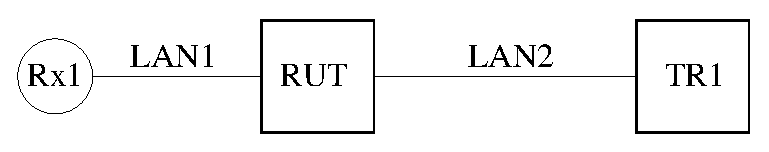
\includegraphics[scale=0.8]{figs/pim_test_2_6_generation_id_option}
    \caption{Generation ID option test setup}
    \label{fig:generation_id_option}
  \end{center}
\end{figure}

\para{Procedure:}

\subpara{Part A: Transmission of a PIM Hello message containing a Generation ID
option.}

\begin{enumerate}

  \item Start the RUT.

  \item Observe the messages transmitted by the RUT on LAN2 for at least
        \verb=Triggered_Hello_Delay= + 3 * \verb=Hello_Holdtime=
        (\ie ({\PimsmTriggeredHelloDelay}) + 3 * ({\PimsmHelloHoldtime})).

  \item Restart the RUT interface that connects the RUT to LAN2.

  \item Observe the messages transmitted by the RUT on LAN2 for at least
        \verb=Triggered_Hello_Delay= ({\PimsmTriggeredHelloDelay}).

  \item Restart the RUT.

  \item Observe the messages transmitted by the RUT on LAN2 for at least
        \verb=Triggered_Hello_Delay= ({\PimsmTriggeredHelloDelay}).

\end{enumerate}

\subpara{Part B: Reception of a PIM Hello message containing a Generation ID
option.}

\begin{enumerate}

  \item Start both the RUT and TR1.

  \item Observe the messages transmitted by the RUT on LAN2.

  \item Quit TR1 (\ie stop it without graceful shutdown), and start it
  immediately.

\end{enumerate}

\subpara{Part C: Reception of a PIM Hello message containing a Generation ID
option when the RUT has pending Join messages to send.}

Configure both the RUT and TR1 such that it is the RP for group
224.0.1.20. This configuration can be either manual, or implicit through the
Bootstrap mechanism. Configure Rx1 such that it is the receiver for group
224.0.1.20.

\begin{enumerate}

  \item Start both the RUT and TR1. If necessary, wait until the RP-set in the
  RUT and TR1 converges.

  \item Start Rx1, and observe the Join state in the RUT and TR1.

  \item Observe the messages transmitted by the RUT on LAN2.

  \item Quit TR1 (\ie stop it without graceful shutdown), and start it
  immediately.

\end{enumerate}

\para{Observable Results:}

\subpara{Part A:}

\begin{itemize}

  \item After the RUT is started, after a random interval between
        0 and \verb=Triggered_Hello_Delay= ({\PimsmTriggeredHelloDelay}) the
        RUT should start transmitting Hello message with Generation ID
        option included. There should be a Hello message every
        \verb=Hello_Holdtime= ({\PimsmHelloHoldtime}), and the value of the
        Generation ID must be same for all messages.

  \item After the RUT interface that connects the RUT to LAN2 is restarted,
        after a random interval between 0 and \verb=Triggered_Hello_Delay=
        ({\PimsmTriggeredHelloDelay}) the RUT should transmit on LAN2 a Hello
        message with Generation ID option included. The value of this
        Generation ID must be different from the value of the Hello message
        before the restart.

  \item After the RUT is restarted,
        after a random interval between 0 and \verb=Triggered_Hello_Delay=
        ({\PimsmTriggeredHelloDelay}) the RUT should transmit on LAN2 a Hello
        message with Generation ID option included. The value of this
        Generation ID must be different from the value of the Hello message
        before the restart.
        
\end{itemize}

\subpara{Part B:}

\begin{itemize}

  \item After the RUT receives the first Hello message from TR1 that
	has different Generation ID from the one before the restart,
        after a random interval between 0 and \verb=Triggered_Hello_Delay=
        ({\PimsmTriggeredHelloDelay}) the RUT should transmit on LAN2 a Hello
        message.

\end{itemize}

\subpara{Part C:}

\begin{itemize}

  \item After the RUT receives the first Hello message from TR1 that
	has different Generation ID from the one before the restart,
	the RUT should transmit immediately on LAN2 a Hello message
	followed by a PIM Join/Prune message with group 224.0.1.20
	included in the list of joined groups.

\end{itemize}

\para{Possible Problems:}
None.

%%%%%%%%%%%%%%%%%%%%%%%%%%%%%%%%%%%%%%%%%%%
\newpage
\section{Two-Way Neighbor Adjacency Without Hello Messages}

\para{Purpose:}
Verify that a router can be configured to form a two-way neighbor adjacency
even if no Hello message was received.

\para{References:}
\begin{itemize}
  \item draft-ietf-pim-sm-v2-new-05 -- Sections 4.3.1, and 4.5
  \item draft-ietf-pim-sm-bsr-02 -- Section 3
\end{itemize}

\para{Discussion:}
The following PIM control messages should only be accepted for processing if
they come from a known PIM neighbor: Join/Prune, Bootstrap, Assert, Graft, and
Graft-Ack. A PIM router hears about PIM neighbors
through PIM Hello messages. However, some older PIM implementations
incorrectly fail to send Hello messages on point-to-point interfaces. Hence,
the spec recommends that a configuration option should be provided to allow
interoperation with such old routers (disabled by default). More specifically,
if the option is enabled, then the above PIM control messages should be
accepted from a neighbor even if no Hello message was received first from that
neighbor.

\para{Test Setup:}
Connect the RUT, TR1, S1, and Rx1 according to
Figure~\ref{fig:two_way_neighbor_adjacency_without_hello_messages}.
Enable PIM-SM on both TR1 and the RUT. Configure TR1
as a Candidate-BSR, and the RUT as a Candidate-RP. Modify or configure TR1
such that it never sends PIM Hello messages. Configure Rx1 and S1 such
that Rx1 is a receiver, and S1 is a sender, both for group 224.0.1.20.

\begin{figure}[htbp]
  \begin{center}
    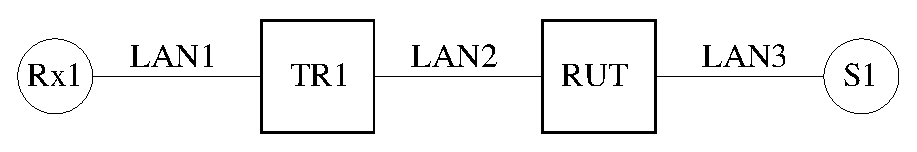
\includegraphics[scale=0.8]{figs/pim_test_2_7_two_way_neighbor_adjacency_without_hello_messages}
    \caption{Two-way neighbor adjacency without Hello messages test
    setup}
    \label{fig:two_way_neighbor_adjacency_without_hello_messages}
  \end{center}
\end{figure}

\para{Procedure:}

\begin{enumerate}

  \item Start TR1 and the RUT.

  \item Observe the messages transmitted by TR1 and the RUT, and the neighbor
  and Bootstrap state information in the RUT.

  \item Wait until TR1 transmits 2-3 Bootstrap messages.

  \item Enable the interoperability option in the RUT (without restarting it),
  such that the RUT would accept PIM control messages from TR1 even if TR1
  does not send Hello messages.

  \item Wait until TR1 transmits 2-3 Bootstrap messages.

  \item Start Rx1.

  \item Start S1.

\end{enumerate}

\para{Observable Results:}

\begin{itemize}

  \item After TR1 and the RUT are started, the RUT should start transmitting
  PIM Hello messages on LAN2.

  \item After TR1 receives the first Hello message from the RUT, TR1 should
  unicast a Bootstrap message to the RUT. After that it start transmitting
  periodically only Bootstrap messages on LAN2.

  \item Each Bootstrap message received by the RUT should be ignored because
  it comes from an unknown neighbor. Therefore, the RUT should not have a
  BSR:

\begin{verbatim}
Xorp> show pim bootstrap
Active zones:
BSR              Pri LocalAddress     Pri State            Timeout SZTimeout
Configured zones:
BSR              Pri LocalAddress     Pri State            Timeout SZTimeout
0.0.0.0            0 0.0.0.0            0 Init                  -1        -1
\end{verbatim}

  In addition, the neighbor state information in the RUT should be empty:

\begin{verbatim}
Xorp> show pim neighbors 
Interface        DRpriority NeighborAddr     V Mode    Holdtime Timeout
\end{verbatim}


  \item After the interoperability option in the RUT is enabled, the next
  Bootstrap message from TR1 should be accepted by the RUT. As a result, the
  Bootstrap state in the RUT should show that TR1 is the BSR:

\begin{verbatim}
Xorp> show pim bootstrap
Active zones:
BSR              Pri LocalAddress     Pri State            Timeout SZTimeout
10.2.0.1           1 0.0.0.0            0 AcceptPreferred       74      1444
\end{verbatim}

  Eventually, the neighbor state information in the RUT may show TR1. If this
  is the case, the state information in the RUT for TR1 should be refreshed by
  each Bootstrap originated by TR1:

\begin{verbatim}
Xorp> show pim neighbors 
Interface        DRpriority NeighborAddr     V Mode    Holdtime Timeout
dc2                    none 10.2.0.1         2 Sparse       210     164
\end{verbatim}

  \item After Rx1 is started, TR1 should send PIM Join message for group
  224.0.1.20 on LAN2 toward the RP (the RUT).

  \item After S1 is started, the multicast data packets originated by it
  should be forwarded by the RUT and TR1 to Rx1.

\end{itemize}

\para{Possible Problems:}
None.


%%%%%%%%%%%%%%%%%%%%%%%%%%%%%%%%%%%%%%%%%%%%%%%%%%%%%%%%%%%%%%%%%%%%%%%
\chapter{PIM Register Messages}

\para{Scope:}
Test sending and receiving of PIM Register messages.

\para{Overview:}
The Designated Router (DR) on a LAN or point-to-point link encapsulates
multicast packets from local sources to the RP for the relevant group
unless it recently received a Register Stop message for that (S,G) or
(*,G) from the RP.  When the DR receives a Register Stop message from
the RP, it starts a Register Stop timer to maintain this state.  Just
before the Register Stop timer expires, the DR sends a Null-Register
message to the RP to allow the RP to refresh the Register Stop
information at the DR.  If the Register Stop timer actually expires, the
DR will resume encapsulating packets from the source to the RP.

%%%%%%%%%%%%%%%%%%%%%%%%%%%%%%%%%%%%%%%%%%%
\newpage
\section{Register Messages Transmission}

\para{Purpose:}
Verify that a DR properly sends Register messages.

\para{References:}
\begin{itemize}
  \item draft-ietf-pim-sm-v2-new-05 -- Section 4.4.1
\end{itemize}

\para{Discussion:}
The DR encapsulates multicast packets from local sources into PIM Register
messages, and unicasts them to the RP for the relevant multicast group.

\para{Test Setup:}
Connect the RUT, TR1, TR2, S1, and Rx1 according to
Figure~\ref{fig:register_messages_transmission}.
Configure the RUT, TR1, and TR2 such that TR1 is the RP for group 224.0.1.20,
and such that it never attempts to switch to the shortest-path tree by
originating an (S,G) SPT Join message toward a source.
Enable PIM-SM on the RUT, TR1, and TR2.
Configure Rx1 and S1 such that Rx1 is a receiver, and S1 is a sender,
both for group 224.0.1.20.


\begin{figure}[htbp]
  \begin{center}
    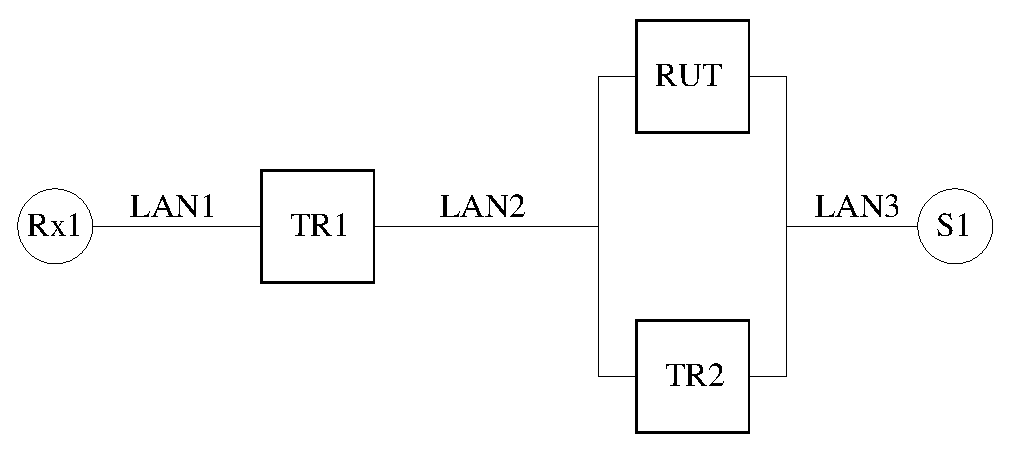
\includegraphics[scale=0.8]{figs/pim_test_3_1_register_messages_transmission}
    \caption{Register messages transmission test setup}
    \label{fig:register_messages_transmission}
  \end{center}
\end{figure}

\para{Procedure:}

\subpara{Part A: Transmission of Register messages.}

\begin{enumerate}

  \item Configure the RUT such that it is the DR on LAN3.

  \item Start the RUT, TR1, and TR2. If necessary, wait until the RP-set in
        the RUT, TR1, and TR1 converges.

  \item Start Rx1.

  \item Observe the messages transmitted by the RUT and TR2 on LAN2.

  \item Start S1.

\end{enumerate}

\subpara{Part B: Non-transmission of Register messages.}

The procedure is same as in Part A, except that TR1 instead of the RUT is the
DR on LAN3.

\subpara{Part C: Switching between transmission and non-transmission of
Register messages.}

\begin{enumerate}

  \item Configure the RUT such that it is the DR on LAN3.

  \item Start the RUT, TR1, and TR2. If necessary, wait until the RP-set in
        the RUT, TR1, and TR1 converges.

  \item Start Rx1.

  \item Observe the messages transmitted by the RUT and TR2 on LAN2.

  \item Start S1.

  \item Reconfigure the RUT (without stopping it), such that TR2 is the DR on
  LAN3.

  \item Reconfigure the RUT (without stopping it), such that it again is the
  DR on LAN3.

\end{enumerate}

\subpara{Part D: Handling of RegisterStop(S,G) messages at the DR.}

\begin{enumerate}

  \item Start the RUT and TR1 (note that in this part we do not use TR2). If
  necessary, wait until the RP-set in the RUT and TR1 converges.

  \item Start Rx1.

  \item Observe the messages transmitted by the RUT on LAN2.

  \item Start S1.

  \item Stop Rx1.

  \item Start Rx1.

\end{enumerate}

\para{Observable Results:}

\subpara{Part A:}

After S1 is started, the RUT should start encapsulating
the data packets transmitted by S1 in PIM Register messages, and unicast them
to the RP (TR1, that should decapsulate and forward them to Rx1).

\subpara{Part B:}

After S1 is started, the RUT should NOT encapsulate the
data packets transmitted by S1 in PIM Register messages. Instead, TR2 should
encapsulate and unicast them to the RP (TR1, that should decapsulate and
forward them to Rx1).

\subpara{Part C:}

\begin{itemize}

  \item After S1 is started, the RUT should start
  encapsulating the data packets transmitted by S1 in PIM Register messages,
  and unicast them to the RP (TR1, that should decapsulate and forward them to
  Rx1).

  \item After the RUT is reconfigured such that it is not the DR on LAN3, it
  should immediately stop transmitting PIM Register messages to the RP.
  Instead, the new DR (TR2) should start transmitting them.

  \item After the RUT is reconfigured such that it is again the DR on LAN3, it
  should immediately start transmitting PIM Register messages to the RP.
  The previous DR (TR2) should stop transmitting them.

\end{itemize}

\subpara{Part D:}

\begin{itemize}

  \item After S1 is started, the RUT should start
  encapsulating the data packets transmitted by S1 in PIM Register messages,
  and unicast them to the RP (TR1, that should decapsulate and forward them to
  Rx1).

  \item After Rx1 is stopped, TR1 should send PIM Register Stop message to
  the RUT for each PIM Register message it receives from the RUT (including
  the PIM Null Register messages). After receiving the first PIM Register Stop
  message, the RUT should stop sending PIM Register messages to the RP (TR1)
  with the encapsulated data packets from S1.
  However, from time to time the RUT should be sending PIM Null Register
  messages to the RP (TR1) with time interval between two messages a random
  value chosen uniformly from the interval \\
  (0.5 * \verb=Register_Suppression_Time=,
  1.5 * \verb=Register_Suppression_Time=) \\
  - \verb=Register_Probe_Time= \\
  = ( (0.5 * {\PimsmRegisterSuppressionTime}, 1.5 *
  {\PimsmRegisterSuppressionTime}) - {\PimsmRegisterProbeTime} ). \\
  To each PIM Null Register message, the RP (TR1) should respond with a PIM
  Register Stop message, therefore the RUT should continue not to encapsulate
  the data packets from S1.

  \item After Rx1 is started again, the RP (TR1) should send an SPT (S,G) Join
  message on LAN2 toward the source. As a result, the data packets from S1
  should be forwarded to the RP (TR1) natively instead of encapsulating them
  in PIM Register messages.

\end{itemize}


\para{Possible Problems:}
In Part C, if the sender's rate is relatively high, there could be few packet
losses at Rx1 when the DR on LAN3 changes.

%%%%%%%%%%%%%%%%%%%%%%%%%%%%%%%%%%%%%%%%%%%
\newpage
\section{Register Tunnel Interface}

\para{Purpose:}
Verify that a Register tunnel virtual interface is properly created, removed,
or changed.

\para{References:}
\begin{itemize}
  \item draft-ietf-pim-sm-v2-new-05 -- Section 4.4.1
\end{itemize}

\para{Discussion:}
When the DR has to encapsulate the data packets from local sources into
PIM Register messages, and unicasts them to the RP for the relevant multicast
group, it creates a Register tunnel virtual interface with its encapsulation
target being the RP. If the DR should stop encapsulating the data packets, it
removes the Register tunnel virtual interface. If the RP for the multicast
group changes, the DR should update the Register tunnel virtual interface.

\para{Test Setup:}
Connect the RUT, TR1, TR2, S1, and Rx1 according to
Figure~\ref{fig:register_tunnel_interface}.
Enable PIM-SM on the RUT, TR1,
and TR2. In all the tests, configure the RP such that it never attempts to
switch to the shortest-path tree by originating an (S,G) SPT Join message
toward a source. Enable PIM-SM on the RUT, TR1, and TR2.  Configure Rx1 and S1
such that Rx1 is a receiver, and S1 is a sender, both for group 224.0.1.20.


\begin{figure}[htbp]
  \begin{center}
    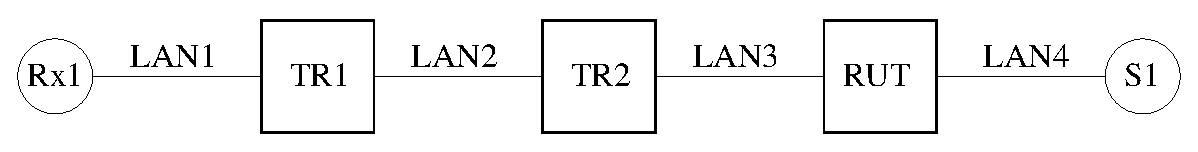
\includegraphics[scale=0.8]{figs/pim_test_3_2_register_tunnel_interface}
    \caption{Register tunnel interface test setup}
    \label{fig:register_tunnel_interface}
  \end{center}
\end{figure}

\para{Procedure:}

\subpara{Part A: Add and remove Register tunnel.}

\begin{enumerate}

  \item Configure TR1 such that it is the RP.

  \item Start the RUT, TR1, and TR2. If necessary, wait until the RP-set in
  the RUT, TR1, and TR2 converges.

  \item Start Rx1.

  \item Observe the Register state machine at the RUT, and the messages
  transmitted by the RUT on LAN3.

  \item Start S1.

  \item Stop Rx1.

  \item Stop S1.

\end{enumerate}

\subpara{Part B: Update Register tunnel.}

\begin{enumerate}

  \item Configure TR1 such that it is the RP.

  \item Start the RUT, TR1, and TR2. If necessary, wait until the RP-set in
  the RUT, TR1, and TR2 converges.

  \item Start Rx1.

  \item Observe the Register state machine at the RUT, and the messages
  transmitted by the RUT on LAN3.

  \item Start S1.

  \item Reconfigure TR1 and TR2 such that TR2 becomes the RP.

\end{enumerate}

\para{Observable Results:}

\subpara{Part A:}

\begin{itemize}

  \item After Rx1 is started, the Register state machine in the RUT for source
  S1 and group 224.0.1.20 should be in No Info state:

\begin{verbatim}
Xorp> show pim join 224.0.1.20
Group           Source          RP              Flags
\end{verbatim}

  Further, no PIM Register messages should be transmitted by the RUT.

  \item After S1 is started, the Register state machine in the RUT for source
  S1 and group 224.0.1.20 should be in Join state, and the Register tunnel
  virtual interface should be created between the RUT and the RP (TR1):

\begin{verbatim}
Xorp> show pim join 224.0.1.20
Group           Source          RP              Flags
224.0.1.20      10.4.0.2        10.2.0.1        SG SPT DirectlyConnectedS 
    Upstream interface (S):   dc0
    Upstream interface (RP):  dc2
    Upstream MRIB next hop (RP): 10.3.0.1
    Upstream MRIB next hop (S):  UNKNOWN
    Upstream RPF'(*,G):       UNKNOWN
    Upstream RPF'(S,G):       UNKNOWN
    Upstream RPF'(S,G,rpt):   UNKNOWN
    Upstream state:           Joined 
    Register state:           RegisterJoin RegisterCouldRegister 
    Join timer:               13
    Local include:            .............
    Local exclude:            .............
    Local include WC:         .............
    Local include SG:         .............
    Local exclude SG:         .............
    Joins RP:                 .............
    Joins WC:                 .............
    Joins SG:                 ............O
    Prunes SG_RPT:            .............
    Join state:               ............O
    Prune state:              .............
    Prune pending state:      .............
    I am assert winner state: .............
    I am assert loser state:  .............
    Assert winner WC:         .............
    Assert winner SG:         .............
    Assert lost WC:           .............
    Could assert SG:          ............O
    I am DR:                  ....O.O......
    Immediate olist RP:       .............
    Immediate olist WC:       .............
    Immediate olist SG:       ............O
    Inherited olist SG:       ............O
    Inherited olist SG_RPT:   .............
    PIM include WC:           .............
\end{verbatim}

  Further, each data packet from S1 should be encapsulated by the RUT in a
  PIM Register message and unicast to the RP (TR1).

  \item After Rx1 is stopped, the RP (TR1) should send PIM Register Stop
  message to the RUT for each PIM Register message it receives from the RUT
  (PIM Null Register messages excluded). After the RUT receives the first
  PIM Register Stop message, the Register tunnel virtual interface to the RP
  (TR1) should be in Prune state:

\begin{verbatim}
Xorp> show pim join 224.0.1.20
Group           Source          RP              Flags
224.0.1.20      10.4.0.2        10.2.0.1        SG DirectlyConnectedS 
    Upstream interface (S):   dc0
    Upstream interface (RP):  dc2
    Upstream MRIB next hop (RP): 10.3.0.1
    Upstream MRIB next hop (S):  UNKNOWN
    Upstream RPF'(*,G):       UNKNOWN
    Upstream RPF'(S,G):       UNKNOWN
    Upstream RPF'(S,G,rpt):   UNKNOWN
    Upstream state:           NotJoined 
    Register state:           RegisterPrune RegisterCouldRegister 
    Join timer:               -1
    Local include:            .............
    Local exclude:            .............
    Local include WC:         .............
    Local include SG:         .............
    Local exclude SG:         .............
    Joins RP:                 .............
    Joins WC:                 .............
    Joins SG:                 .............
    Prunes SG_RPT:            .............
    Join state:               .............
    Prune state:              .............
    Prune pending state:      .............
    I am assert winner state: .............
    I am assert loser state:  .............
    Assert winner WC:         .............
    Assert winner SG:         .............
    Assert lost WC:           .............
    Could assert SG:          .............
    I am DR:                  ....O.O......
    Immediate olist RP:       .............
    Immediate olist WC:       .............
    Immediate olist SG:       .............
    Inherited olist SG:       .............
    Inherited olist SG_RPT:   .............
    PIM include WC:           .............
\end{verbatim}

  Further, from time to time the RUT should be sending PIM Null Register
  messages to the RP (TR1) with time interval between two messages a random
  value chosen uniformly from the interval \\
  (0.5 * \verb=Register_Suppression_Time=,
  1.5 * \verb=Register_Suppression_Time=) \\
  - \verb=Register_Probe_Time= \\
  = ( (0.5 * {\PimsmRegisterSuppressionTime}, 1.5 *
  {\PimsmRegisterSuppressionTime}) - {\PimsmRegisterProbeTime} ).\\
  To each PIM Null Register message, TR1 should respond with a PIM Register
  Stop message, therefore the RUT should continue not to encapsulate the data
  packets from S1.

  \item After S1 is stopped, and after period of \verb=Keepalive_Period=
  ({\PimsmKeepalivePeriod}), the state for source S1 and group 224.0.1.20
  in the RUT should expire:

\begin{verbatim}
Xorp> show pim join 224.0.1.20
Group           Source          RP              Flags
\end{verbatim}

  Further, no PIM Register messages should be transmitted by the RUT.

\end{itemize}

\subpara{Part B:}

\begin{itemize}

  \item The results until after S1 is started should be same as in Part A.

  \item After TR1 and TR2 are reconfigured such that TR2 becomes the RP,
  and after the RP-set in the RUT, TR1, and TR2 converges, the Register tunnel
  virtual interface in the RUT should be updated to point to the new RP (TR2).
  The Register state machine should still be in Join state:

\begin{verbatim}
Xorp> show pim join 224.0.1.20
Group           Source          RP              Flags
224.0.1.20      10.4.0.2        10.3.0.1        SG SPT DirectlyConnectedS 
    Upstream interface (S):   dc0
    Upstream interface (RP):  dc2
    Upstream MRIB next hop (RP): 10.3.0.1
    Upstream MRIB next hop (S):  UNKNOWN
    Upstream RPF'(*,G):       UNKNOWN
    Upstream RPF'(S,G):       UNKNOWN
    Upstream RPF'(S,G,rpt):   UNKNOWN
    Upstream state:           Joined 
    Register state:           RegisterJoin RegisterCouldRegister 
    Join timer:               48
    Local include:            .............
    Local exclude:            .............
    Local include WC:         .............
    Local include SG:         .............
    Local exclude SG:         .............
    Joins RP:                 .............
    Joins WC:                 .............
    Joins SG:                 ............O
    Prunes SG_RPT:            .............
    Join state:               ............O
    Prune state:              .............
    Prune pending state:      .............
    I am assert winner state: .............
    I am assert loser state:  .............
    Assert winner WC:         .............
    Assert winner SG:         .............
    Assert lost WC:           .............
    Could assert SG:          ............O
    I am DR:                  ....O.O......
    Immediate olist RP:       .............
    Immediate olist WC:       .............
    Immediate olist SG:       ............O
    Inherited olist SG:       ............O
    Inherited olist SG_RPT:   .............
    PIM include WC:           .............
\end{verbatim}

  Further, each data packet from S1 should be encapsulated by the RUT in a PIM
  Register message and unicast to the new RP (TR2).

\end{itemize}


\para{Possible Problems:}
In Part B, if the RP-set converges such that the RUT learns that TR2 is the RP
before TR2 itself, the PIM Register messages the RUT sends to TR2 may result
in TR2 sending-back PIM Register Stop messages. Those PIM Register Stop
messages would change the state for source S1 and group 224.0.1.20 in the RUT
to Prune, and will stop the PIM Register encapsulation of the data packets
from S1. Further, after TR2 learns that it is the RP, it may actually send an
SPT (S,G) Join message on LAN2 toward the source. As a result, the data
packets from S1 will be forwarded to Rx1 natively instead of encapsulating
them in PIM Register messages.

%%%%%%%%%%%%%%%%%%%%%%%%%%%%%%%%%%%%%%%%%%%
\newpage
\section{Register Messages Reception}

\para{Purpose:}
Verify that an RP properly receives and decapsulates Register messages.

\para{References:}
\begin{itemize}
  \item draft-ietf-pim-sm-v2-new-05 -- Section 4.4.2
\end{itemize}

\para{Discussion:}
If the RP for a multicast group receives Register messages for that group,
and if there are receivers that have joined that group, the RP decapsulates
the data packets, and forwards them natively to the receivers. If the
multicast group has no receivers, the RP sends Register Stop to the originator
of the Register messages.

\para{Test Setup:}
Connect the RUT, TR1, TR2, S1, and Rx1 according to
Figure~\ref{fig:register_messages_reception}.
Enable PIM-SM on the RUT,
TR1, and TR2. In all the tests, configure the RP such that it never attempts to
switch to the shortest-path tree by originating an (S,G) SPT Join message
toward a source. Enable PIM-SM on the RUT, TR1, and TR2.  Configure Rx1 and S1
such that Rx1 is a receiver, and S1 is a sender, both for group 224.0.1.20.


\begin{figure}[htbp]
  \begin{center}
    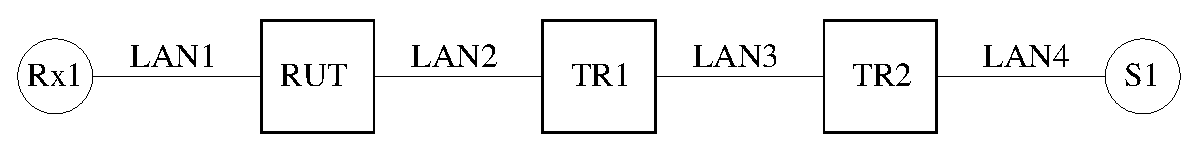
\includegraphics[scale=0.8]{figs/pim_test_3_3_register_messages_reception}
    \caption{Register messages reception test setup}
    \label{fig:register_messages_reception}
  \end{center}
\end{figure}

\para{Procedure:}

\subpara{Part A: Receiving Register messages at the RP when there is a
receiver.}

\begin{enumerate}

  \item Configure the RUT such that it is the RP.

  \item Start the RUT, TR1, and TR2. If necessary, wait intil the RP-set in
  the RUT, TR1, and TR2 converges.

  \item Start Rx1.

  \item Observe the messages transmitted by the RUT on LAN2, and the messages
  received by Rx1.

  \item Start S1.

  \item Stop Rx1.

  \item Start Rx1.

\end{enumerate}

\subpara{Part B: Receiving Register messages at the RP when there is no
receiver.}

\begin{enumerate}

  \item Configure the RUT such that it is the RP.

  \item Start the RUT, TR1, and TR2. If necessary, wait intil the RP-set in
  the RUT, TR1, and TR2 converges.

  \item Observe the messages transmitted by the RUT on LAN2, and the messages
  received by Rx1.

  \item Start S1.

  \item Start Rx1.

  \item Stop Rx1.

  \item Start Rx1.

\end{enumerate}

\subpara{Part C: Receiving Register messages at the non-RP.}

\begin{enumerate}

  \item Manually configure TR2 only to appears that the RUT is the
  RP. However, configure the RUT itself, and TR1 such that for both of them
  appear that TR1 is the RP.

  \item Start Rx1.

  \item Start S1.

\end{enumerate}


\para{Observable Results:}

\subpara{Part A:}

\begin{itemize}

  \item After S1 is started, the data messages it transmits should be
  encapsulated in PIM Register messages by TR2, and sent to the RP (the
  RUT). The RUT should decapsulate them, and forward the inner multicast
  packets down the shared multicast tree to Rx1.

  \item After Rx1 is stopped, the RUT should send PIM Register Stop message to
  TR2 for each PIM Register message it receives from the RUT (including
  the PIM Null Register messages). After receiving the first PIM Register Stop
  message, TR2 should stop sending PIM Register messages to the RP (the RUT)
  with the encapsulated data packets from S1.
  However, from time to time TR2 should be sending PIM Null Register
  messages to the RP (the RUT) with time interval between two messages a random
  value chosen uniformly from the interval \\
  (0.5 * \verb=Register_Suppression_Time=,
  1.5 * \verb=Register_Suppression_Time=) \\
  - \verb=Register_Probe_Time= \\
  = ( (0.5 * {\PimsmRegisterSuppressionTime}, 1.5 *
  {\PimsmRegisterSuppressionTime}) - {\PimsmRegisterProbeTime} ). \\
  To each PIM Null Register message, the RP (the RUT) should respond with a
  PIM Register Stop message, therefore TR2 should continue not to
  encapsulate the data packets from S1.

  \item After Rx1 is started again, the RUT should send an SPT (S,G) Join
  message on LAN2 toward the source. As a result, the data packets from S1
  should be forwarded to the RP (the RUT) natively instead of encapsulating
  them in PIM Register messages.

\end{itemize}

\subpara{Part B:}

\begin{itemize}

  \item After S1 is started, the first one or few data messages it transmits
  should be encapsulated in PIM Register messages by TR2, and sent to the RP
  (the RUT). The RUT should respond to each PIM Register message with a PIM
  Register Stop message for source S1 and group 224.0.1.20. After TR2 receives
  the first Register Stop message, it should stop encapsulating the data
  packets and sending them to the RP (the RUT).

  \item From time to time TR2 should be sending PIM Null Register
  messages to the RP (the RUT) with time interval between two messages a random
  value chosen uniformly from the interval \\
  (0.5 * \verb=Register_Suppression_Time=,
  1.5 * \verb=Register_Suppression_Time=) \\
  - \verb=Register_Probe_Time= \\
  = ( (0.5 * {\PimsmRegisterSuppressionTime}, 1.5 *
  {\PimsmRegisterSuppressionTime}) - {\PimsmRegisterProbeTime} ). \\
  To each PIM Null Register message, the RP (the RUT) should respond with a
  PIM Register Stop message, therefore TR2 should continue not to
  encapsulate the data packets from S1.

  \item After Rx1 is started, the RUT should send an SPT (S,G) Join message
  on LAN2 toward the source. As a result, the data packets from S1 should be
  forwarded to the RP (the RUT) natively instead of encapsulating them in PIM
  Register messages.

  \item After Rx1 is stopped, the RUT should send an SPT (S,G) Prune message
  on LAN2 toward the source. As a result, the data packets from S1 should not
  be forwarded by TR2 from LAN4 on LAN3.

  \item After Rx1 is started again, the RUT should send an SPT (S,G) Join
  message on LAN2 toward the source. As a result, the data packets from S1
  should be again be forwarded to the RP (the RUT) natively instead of
  encapsulating them in PIM Register messages.

\end{itemize}

\subpara{Part C:}

\begin{itemize}

  \item After S1 is started, the first one or few data messages it transmits
  should be encapsulated in PIM Register messages by TR2, and sent to the RUT,
  which TR2 thinks is the RP for group 224.0.1.20.
  However, because the RUT is not the RP, it should respond to each PIM
  Register message with a PIM Register Stop message for source S1 and group
  224.0.1.20. After TR2 receives the first Register Stop message, it should
  stop encapsulating the data packets and sending them to the RUT.

  \item From time to time TR2 should be sending PIM Null Register
  messages to the RUT with time interval between two messages a random
  value chosen uniformly from the interval \\
  (0.5 * \verb=Register_Suppression_Time=,
  1.5 * \verb=Register_Suppression_Time=) \\
  - \verb=Register_Probe_Time= \\
  = ( (0.5 * {\PimsmRegisterSuppressionTime}, 1.5 *
  {\PimsmRegisterSuppressionTime}) - {\PimsmRegisterProbeTime} ). \\
  To each PIM Null Register message, the RUT should respond with a
  PIM Register Stop message, therefore TR2 should continue not to
  encapsulate the data packets from S1.

\end{itemize}

\para{Possible Problems:}
None.


%%%%%%%%%%%%%%%%%%%%%%%%%%%%%%%%%%%%%%%%%%%%%%%%%%%%%%%%%%%%%%%%%%%%%%%
\chapter{PIM Join/Prune Messages}

\para{Scope:}
Test sending and receiving of PIM Join/Prune messages.

\para{Overview:}
A PIM Join/Prune message consists of a list of groups and a list of
Joined and Pruned source for each group. It is used by the router
originating it to express interest (or lack of interest) in receiving
multicast traffic for specific groups and sources.

A Join/Prune message may contain four types of entries. An (*,G)
Join/Prune entry is sent toward the RP for group G, and is used to
express interest in receiving multicast packets from all sources for
that group. An (S,G) Join/Prune entry is sent toward the specified
source S, and is used to express interest in receiving multicast packets
from the specified source S and group G. An (S,G,rpt) Prune entry is
sent toward the RP for group G, and is used to stop receiving multicast
packets on the shared tree for the specified source S (note that there
is no (S,G,rpt) Join entry, because the (*,G) entry is used for that
purpose). An (*,*,RP) Join/Prune entry is sent toward the specified RP,
and is used to express interest in receiving multicast packets for all
multicast groups that use the specified RP as the root of their shared
trees.

The Join/Prune messages are sent either periodic or are triggered by
some events. Typically, all Join messages and the (S,G,rpt) Prune
messages are sent periodically.

%%%%%%%%%%%%%%%%%%%%%%%%%%%%%%%%%%%%%%%%%%%
\newpage
\section{Receiving (*,*,RP) Join/Prune Messages}

\para{Purpose:}
Verify that (*,*,RP) Join/Prune messages are received and processed
properly.

\para{References:}
\begin{itemize}
  \item draft-ietf-pim-sm-v2-new-05 -- Section 4.5.1
\end{itemize}

\para{Discussion:}
When a PIM-SM router receives a PIM (*,*,RP) Join/Prune message, the
per-interface (*,*,RP) state-machine should be updated appropriately.
Typically, if an (*,*,RP) Join message is received, the interface it was
received on should be added to the set of outgoing interfaces to
forward packets destined for any group handled by the specified RP.
If that set has just became non-empty, an (*,*,RP) Join should be sent
toward the RP.
If an (*,*,RP) Prune message is received, typically it should remove
the interface it was received on from the set of outgoing interfaces
to forward packets destined to any group handled by the specified RP. If
that set has just became empty, an (*,*,RP) Prune message should be
sent toward the RP.

\para{Test Setup:}
Connect the RUT, TR1, TR2, TR3, S1, and S2 according to
Figure~\ref{fig:receiving_rp_join_prune_messages}~\footnote{Note that S1 is
used only when TR3 and S2 are not used, hence it is not necessary to have two
senders at same time.}.
Enable PIM-SM on the RUT, TR1, TR2, and TR3.
Configure S1 and S2 as senders for group 224.0.1.20.

\begin{figure}[htbp]
  \begin{center}
    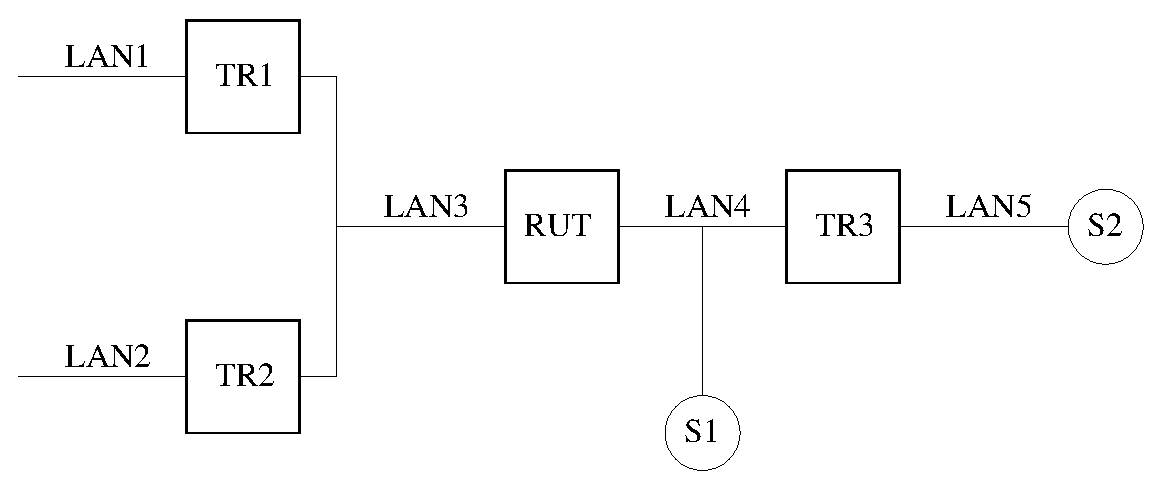
\includegraphics[scale=0.8]{figs/pim_test_4_1_receiving_rp_join_prune_messages}
    \caption{Receiving (*,*,RP) Join/Prune messages test setup}
    \label{fig:receiving_rp_join_prune_messages}
  \end{center}
\end{figure}

\para{Procedure:}

\subpara{Part A: Receiving (*,*,RP) Join messages at the RP.}

\begin{enumerate}

  \item Configure the RUT as the RP. Start the RUT and TR1. If
  necessary, wait until the RP-set in the RUT and TR1 converges.

  \item Start observing the downstream (*,*,RP) per-interface state
  machine at the RUT.

  \item Compose an (*,*,RP) Join message at TR1 with the RP address set
  to the address of the RUT, and send it to the RUT.
  The \verb=J/P_HoldTime= of the message should be set to its default
  value ({\PimsmJPHoldTime}).

  \item Start S1, and observe the data packets transmitted by the RUT on
  LAN3.

  \item Wait until the downstream (*,*,RP) per-interface state in the RUT
  expires.

  \item Observe the data packets transmitted by the RUT on LAN3.

\end{enumerate}

\subpara{Part B: Receiving (*,*,RP) Prune messages at the RP.}

\begin{enumerate}

  \item Configure the RUT as the RP. Start the RUT and TR1. If
  necessary, wait until the RP-set in the RUT and TR1 converges.

  \item Start observing the downstream (*,*,RP) per-interface state
  machine at the RUT.

  \item Compose an (*,*,RP) Prune message at TR1 with the RP address set
  to the address of the RUT, and send it to the RUT.
  The \verb=J/P_HoldTime= of the message should be set to its default
  value ({\PimsmJPHoldTime}).

  \item Compose an (*,*,RP) Join message at TR1 with the RP address set
  to the address of the RUT, and send it to the RUT.
  The \verb=J/P_HoldTime= of the message should be set to its default
  value ({\PimsmJPHoldTime}).

  \item Start S1, and observe the data packets transmitted by the RUT on
  LAN3.

  \item Compose an (*,*,RP) Prune message at TR1 with the RP address set
  to the address of the RUT, and send it to the RUT.

  \item Observe the messages and data packets transmitted by the RUT on
  LAN3.

\end{enumerate}

\subpara{Part C: Receiving (*,*,RP) Join messages at non-RP router.}

\begin{enumerate}

  \item Configure TR3 as the RP. Start the RUT, TR1, and TR3. If
  necessary, wait until the RP-set in the RUT, TR1, and TR3
  converges.

  \item Start observing the downstream (*,*,RP) per-interface state
  machine at the RUT.

  \item Compose an (*,*,RP) Join message at TR1 with the RP address set
  to the address of TR3, and send it to the RUT.
  The \verb=J/P_HoldTime= of the message should be set to its default
  value ({\PimsmJPHoldTime}).

  \item Observe the messages transmitted by the RUT on LAN4.

  \item Start S2, and observe the data packets transmitted by the RUT on
  LAN3.

  \item Wait until the downstream (*,*,RP) per-interface state in the RUT
  expires.

  \item Observe the data packets transmitted by the RUT on LAN3.

\end{enumerate}

\subpara{Part D: Receiving (*,*,RP) Prune messages at non-RP router.}

\begin{enumerate}

  \item Configure TR3 as the RP. Start the RUT, TR1, and TR3. If
  necessary, wait until the RP-set in the RUT, TR1, and TR3
  converges.

  \item Start observing the downstream (*,*,RP) per-interface state
  machine at the RUT.

  \item Compose an (*,*,RP) Prune message at TR1 with the RP address set
  to the address of TR3, and send it to the RUT.
  The \verb=J/P_HoldTime= of the message should be set to its default
  value ({\PimsmJPHoldTime}).

  \item Compose an (*,*,RP) Join message at TR1 with the RP address set
  to the address of TR3, and send it to the RUT.
  The \verb=J/P_HoldTime= of the message should be set to its default
  value ({\PimsmJPHoldTime}).

  \item Observe the messages transmitted by the RUT on LAN4.

  \item Start S2, and observe the data packets transmitted by the RUT on
  LAN3.

  \item Compose an (*,*,RP) Prune message at TR1 with the RP address set
  to the address of TR3, and send it to the RUT.

  \item Observe the messages transmitted by the RUT on LAN3 and LAN4,
  and the data packets transmitted by the RUT on LAN3.

\end{enumerate}

\subpara{Part E: Receiving (*,*,RP) Prune messages on a LAN.}

This part is same as Part D, except that in Step 1 we start TR2 as well.

\subpara{Part F: Receiving (*,*,RP) Join and Prune messages on a LAN.}

This part is same as Part E, except that in Step 2 we compose and send
same (*,*,RP) Join message from TR2 as well.

\para{Observable Results:}

\subpara{Part A:}

\begin{itemize}

  \item After the (*,*,RP) Join message is received by the RUT, it
  should create the appropriate (*,*,RP) multicast routing entry for
  that RP, and the interface toward LAN3 should be in Join state and
  added to the set of outgoing interface for that entry:

\begin{verbatim}
Xorp> show pim join 
Group           Source          RP              Flags
224.0.0.0       10.3.0.1        10.3.0.1        RP   
    Upstream interface (S):   UNKNOWN
    Upstream interface (RP):  register_vif
    Upstream MRIB next hop (RP): UNKNOWN
    Upstream MRIB next hop (S):  UNKNOWN
    Upstream RPF'(*,G):       UNKNOWN
    Upstream RPF'(S,G):       UNKNOWN
    Upstream RPF'(S,G,rpt):   UNKNOWN
    Upstream state:           Joined 
    Register state:           
    Join timer:               52
    Local include:            ..............
    Local exclude:            ..............
    Local include WC:         ..............
    Local include SG:         ..............
    Local exclude SG:         ..............
    Joins RP:                 ......O.......
    Joins WC:                 ..............
    Joins SG:                 ..............
    Prunes SG_RPT:            ..............
    Join state:               ......O.......
    Prune state:              ..............
    Prune pending state:      ..............
    I am assert winner state: ..............
    I am assert loser state:  ..............
    Assert winner WC:         ..............
    Assert winner SG:         ..............
    Assert lost WC:           ..............
    Could assert SG:          ..............
    I am DR:                  .....OO.......
    Immediate olist RP:       ......O.......
    Immediate olist WC:       ..............
    Immediate olist SG:       ..............
    Inherited olist SG:       ..............
    Inherited olist SG_RPT:   ..............
    PIM include WC:           ..............
\end{verbatim}

  \item After S1 is started, the multicast data packets should be
  forwarded by the RUT on LAN3.

  \item After \verb=J/P_HoldTime= ({\PimsmJPHoldTime}),
  the (*,*,RP) state machine for the interface that connects the RUT to
  LAN3 should timeout and transition to NoInfo state
  (\ie the (*,*,RP) state in the RUT should expire).
  As a result of that transition, no multicast packets should be
  forwarded by the RUT on LAN3.

\end{itemize}

\subpara{Part B:}

\begin{itemize}

  \item After the (*,*,RP) Prune message is received by the RUT,
  the (*,*,RP) state machine for the interface that connects the RUT to
  LAN3 should continue to stay in the NoInfo state (\ie no (*,*,RP) multicast
  routing entry should be created).
  
  \item After that, the results until after S1 is started should be same as in
  Part A.

  \item After the (*,*,RP) Prune message is received by the RUT,
  the (*,*,RP) state machine for the interface that connects the RUT to
  LAN3 should transition to NoInfo state
  (\ie the (*,*,RP) state in the RUT should expire).
  As a result of that transition no multicast packets should be
  forwarded by the RUT on LAN3.

\end{itemize}

\subpara{Part C:}

\begin{itemize}

  \item After the (*,*,RP) Join message is received by the RUT, it
  should create the appropriate (*,*,RP) multicast routing entry for
  that RP, and the interface toward LAN3 should be in Join state and
  added to the set of outgoing interface for that entry:

\begin{verbatim}
Xorp> show pim join 
Group           Source          RP              Flags
224.0.0.0       10.9.0.1        10.9.0.1        RP   
    Upstream interface (S):   UNKNOWN
    Upstream interface (RP):  dc1
    Upstream MRIB next hop (RP): 10.3.0.2
    Upstream MRIB next hop (S):  UNKNOWN
    Upstream RPF'(*,G):       UNKNOWN
    Upstream RPF'(S,G):       UNKNOWN
    Upstream RPF'(S,G,rpt):   UNKNOWN
    Upstream state:           Joined 
    Register state:           
    Join timer:               47
    Local include:            ..............
    Local exclude:            ..............
    Local include WC:         ..............
    Local include SG:         ..............
    Local exclude SG:         ..............
    Joins RP:                 ......O.......
    Joins WC:                 ..............
    Joins SG:                 ..............
    Prunes SG_RPT:            ..............
    Join state:               ......O.......
    Prune state:              ..............
    Prune pending state:      ..............
    I am assert winner state: ..............
    I am assert loser state:  ..............
    Assert winner WC:         ..............
    Assert winner SG:         ..............
    Assert lost WC:           ..............
    Could assert SG:          ..............
    I am DR:                  ......O.......
    Immediate olist RP:       ......O.......
    Immediate olist WC:       ..............
    Immediate olist SG:       ..............
    Inherited olist SG:       ..............
    Inherited olist SG_RPT:   ..............
    PIM include WC:           ..............
\end{verbatim}

  Further, the RUT itself should originate an (*,*,RP) Join message
  toward the RP (TR3).

  \item After S2 is started, the multicast data packets forwarded by TR3
  on LAN4 should be forwarded by the RUT on LAN3.

  \item After \verb=J/P_HoldTime= ({\PimsmJPHoldTime}),
  the (*,*,RP) state machine for the interface that connects the RUT to
  LAN3 should timeout and transition to NoInfo state
  (\ie the (*,*,RP) state in the RUT should expire).
  As a result of that transition, the RUT should send (*,*,RP) Prune
  message toward the RP (TR3), and no multicast packets should be
  forwarded by the RUT on LAN3.

\end{itemize}

\subpara{Part D:}

\begin{itemize}

  \item After the (*,*,RP) Prune message is received by the RUT,
  the (*,*,RP) state machine for the interface that connects the RUT to
  LAN3 should continue to stay in the NoInfo state (\ie no (*,*,RP) multicast
  routing entry should be created).

  \item After that, the results until after S2 is started should be same as in
  Part C.

  \item After the (*,*,RP) Prune message from TR1 is received by the RUT,
  the (*,*,RP) state machine for the interface that connects the RUT to
  LAN3 should transition to NoInfo state
  (\ie the (*,*,RP) state in the RUT should expire).
  As a result of that transition, the RUT should send (*,*,RP) Prune
  message toward the RP (TR3), and no multicast packets should be
  forwarded by the RUT on LAN3. Note that because the RUT has only one
  PIM neighbor on LAN3, it does not need to send (*,*,RP) PruneEcho on
  LAN3.

\end{itemize}

\subpara{Part E:}

\begin{itemize}

  \item The results until after S2 is started should be same as in
  Part C and D.

  \item After the (*,*,RP) Prune message from TR1 is received by the RUT,
  the (*,*,RP) state machine for the interface that connects the RUT to
  LAN3 should transition to PrunePending state (the reason that it does
  not transit to NoInfo instead is because the RUT has more than one PIM
  neighbors on that interface).
  After \verb=J/P_Override_Interval(I)= (\PimsmJPOverrideIntervalI),
  the PrunePending timer on that interface should expire, and the
  (*,*,RP) state machine for the interface should send (*,*,RP) PruneEcho
  on LAN3 and transit to NoInfo
  state (\ie the (*,*,RP) state in the RUT should expire).
  As a result of that transition, the RUT should send (*,*,RP) Prune
  message toward the RP (TR3), and no multicast packets should be
  forwarded by the RUT on LAN3.

\end{itemize}

\subpara{Part F:}

\begin{itemize}

  \item The results until after S2 is started should be same as in
  Part C, D, and E.

  \item After the (*,*,RP) Prune message from TR1 is received by the RUT,
  the (*,*,RP) state machine for the interface that connects the RUT to
  LAN3 should transition to PrunePending state (the reason that it does
  not transit to NoInfo instead is because the RUT has more than one PIM
  neighbors on that interface).
  Assuming that TR2 has (*,*,RP) multicast routing entry in Joined state
  for the RP it had originated (*,*,RP) Join message earlier, then after
  very short random interval \verb=t_override= ({\PimsmTOverride}) TR2
  should send another (*,*,RP) Join message to the RUT.
  After the RUT receives that (*,*,RP) Join message from TR2,
  the (*,*,RP) state machine for the interface that connects the RUT to
  LAN3 should transition back to Join state.
  As a result of that transition, the RUT should not send (*,*,RP) Prune
  message toward the RP (TR3), and the multicast packets should continue
  to be forwarded by the RUT on LAN3.

\end{itemize}

\para{Possible Problems:}
None.

%%%%%%%%%%%%%%%%%%%%%%%%%%%%%%%%%%%%%%%%%%%
\newpage
\section{Receiving (*,G) Join/Prune Messages}

\para{Purpose:}
Verify that (*,G) Join/Prune messages are received and processed
properly.

\para{References:}
\begin{itemize}
  \item draft-ietf-pim-sm-v2-new-05 -- Section 4.5.2
\end{itemize}

\para{Discussion:}
When a PIM-SM router receives a PIM (*,G) Join/Prune message, the
per-interface (*,G) state-machine should be updated appropriately.
Typically, if an (*,G) Join message is received, the interface it was
received on should be added to the set of outgoing interfaces to
forward packets destined for the specified multicast group address.
If that set has just became non-empty, an (*,G) Join should be sent
toward the RP for that group.
If an (*,G) Prune message is received, typically it should remove
the interface it was received on from the set of outgoing interfaces
for that group. If
that set has just became empty, an (*,G) Prune message should be
sent toward the RP for that group.

\para{Test Setup:}
Connect the RUT, TR1, TR2, TR3, S1, and S2 according to
Figure~\ref{fig:receiving_wc_join_prune_messages}~\footnote{Note that S1 is
used only when TR3 and S2 are not used, hence it is not necessary to have two
senders at same time.}.
Enable PIM-SM on the RUT, TR1, TR2, and TR3.
Configure S1 and S2 as senders for group 224.0.1.20.

\begin{figure}[htbp]
  \begin{center}
    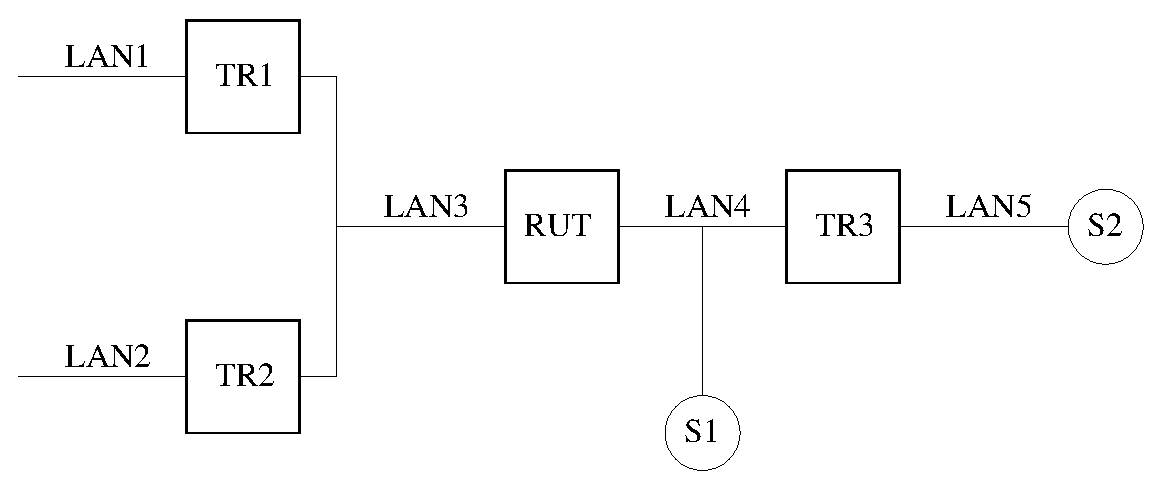
\includegraphics[scale=0.8]{figs/pim_test_4_2_receiving_wc_join_prune_messages}
    \caption{Receiving (*,G) Join/Prune messages test setup}
    \label{fig:receiving_wc_join_prune_messages}
  \end{center}
\end{figure}

\para{Procedure:}

\subpara{Part A: Receiving (*,G) Join messages at the RP.}

\begin{enumerate}

  \item Configure the RUT as the RP. Start the RUT and TR1. If
  necessary, wait until the RP-set in the RUT and TR1 converges.

  \item Start observing the downstream (*,G) per-interface state
  machine at the RUT.

  \item Compose an (*,G) Join message at TR1 with the RP address set
  to the address of the RUT, and send it to the RUT.
  The \verb=J/P_HoldTime= of the message should be set to its default
  value ({\PimsmJPHoldTime}).

  \item Start S1, and observe the data packets transmitted by the RUT on
  LAN3.

  \item Wait until the downstream (*,G) per-interface state in the RUT
  expires.

  \item Observe the data packets transmitted by the RUT on LAN3.

\end{enumerate}

\subpara{Part B: Receiving (*,G) Prune messages at the RP.}

\begin{enumerate}

  \item Configure the RUT as the RP. Start the RUT and TR1. If
  necessary, wait until the RP-set in the RUT and TR1 converges.

  \item Start observing the downstream (*,G) per-interface state
  machine at the RUT.

  \item Compose an (*,G) Prune message at TR1 with the RP address set
  to the address of the RUT, and send it to the RUT.
  The \verb=J/P_HoldTime= of the message should be set to its default
  value ({\PimsmJPHoldTime}).

  \item Compose an (*,G) Join message at TR1 with the RP address set
  to the address of the RUT, and send it to the RUT.
  The \verb=J/P_HoldTime= of the message should be set to its default
  value ({\PimsmJPHoldTime}).

  \item Start S1, and observe the data packets transmitted by the RUT on
  LAN3.

  \item Compose an (*,G) Prune message at TR1 with the RP address set
  to the address of the RUT, and send it to the RUT.

  \item Observe the messages and data packets transmitted by the RUT on
  LAN3.

\end{enumerate}

\subpara{Part C: Receiving (*,G) Join messages at non-RP router.}

\begin{enumerate}

  \item Configure TR3 as the RP. Start the RUT, TR1, and TR3. If
  necessary, wait until the RP-set in the RUT, TR1, and TR3
  converges.

  \item Start observing the downstream (*,G) per-interface state
  machine at the RUT.

  \item Compose an (*,G) Join message at TR1 with the RP address set
  to the address of TR3, and send it to the RUT.
  The \verb=J/P_HoldTime= of the message should be set to its default
  value ({\PimsmJPHoldTime}).

  \item Observe the messages transmitted by the RUT on LAN4.

  \item Start S2, and observe the data packets transmitted by the RUT on
  LAN3.

  \item Wait until the downstream (*,G) per-interface state in the RUT
  expires.

  \item Observe the data packets transmitted by the RUT on LAN3.

\end{enumerate}

\subpara{Part D: Receiving (*,G) Prune messages at non-RP router.}

\begin{enumerate}

  \item Configure TR3 as the RP. Start the RUT, TR1, and TR3. If
  necessary, wait until the RP-set in the RUT, TR1, and TR3
  converges.

  \item Start observing the downstream (*,G) per-interface state
  machine at the RUT.

  \item Compose an (*,G) Prune message at TR1 with the RP address set
  to the address of TR3, and send it to the RUT.
  The \verb=J/P_HoldTime= of the message should be set to its default
  value ({\PimsmJPHoldTime}).

  \item Compose an (*,G) Join message at TR1 with the RP address set
  to the address of TR3, and send it to the RUT.
  The \verb=J/P_HoldTime= of the message should be set to its default
  value ({\PimsmJPHoldTime}).

  \item Observe the messages transmitted by the RUT on LAN4.

  \item Start S2, and observe the data packets transmitted by the RUT on
  LAN3.

  \item Compose an (*,G) Prune message at TR1 with the RP address set
  to the address of TR3, and send it to the RUT.

  \item Observe the messages transmitted by the RUT on LAN3 and LAN4,
  and the data packets transmitted by the RUT on LAN3.

\end{enumerate}

\subpara{Part E: Receiving (*,G) Prune messages on a LAN.}

This part is same as Part D, except that in Step 1 we start TR2 as well.

\subpara{Part F: Receiving (*,G) Join and Prune messages on a LAN.}

This part is same as Part E, except that in Step 2 we compose and send
same (*,G) Join message from TR2 as well.

\subpara{Part G: Receiving (*,G) Join messages with mismatch RP address at
non-RP router}

\begin{enumerate}

  \item Configure TR3 as the RP. Start the RUT, TR1, and TR3. If
  necessary, wait until the RP-set in the RUT, TR1, and TR3
  converges.

  \item Start observing the downstream (*,G) per-interface state
  machine at the RUT.

  \item Compose an (*,G) Join message at TR1 with the RP address set
  to an address that is different from the address of TR3, but such that
  TR3 is the next-hop router toward it (\eg the address of S), and send it to
  the RUT.
  The \verb=J/P_HoldTime= of the message should be set to its default
  value ({\PimsmJPHoldTime}).

  \item Observe the messages transmitted by the RUT on LAN4.

\end{enumerate}

\para{Observable Results:}

\subpara{Part A:}

\begin{itemize}

  \item After the (*,G) Join message is received by the RUT, it
  should create the appropriate (*,G) multicast routing entry for
  that group, and the interface toward LAN3 should be in Join state and
  added to the set of outgoing interface for that entry:

\begin{verbatim}
Xorp> show pim join 
Group           Source          RP              Flags
224.0.1.20      0.0.0.0         10.3.0.1        WC   
    Upstream interface (S):   UNKNOWN
    Upstream interface (RP):  register_vif
    Upstream MRIB next hop (RP): UNKNOWN
    Upstream MRIB next hop (S):  UNKNOWN
    Upstream RPF'(*,G):       UNKNOWN
    Upstream RPF'(S,G):       UNKNOWN
    Upstream RPF'(S,G,rpt):   UNKNOWN
    Upstream state:           Joined 
    Register state:           
    Join timer:               42
    Local include:            ..............
    Local exclude:            ..............
    Local include WC:         ..............
    Local include SG:         ..............
    Local exclude SG:         ..............
    Joins RP:                 ..............
    Joins WC:                 ......O.......
    Joins SG:                 ..............
    Prunes SG_RPT:            ..............
    Join state:               ......O.......
    Prune state:              ..............
    Prune pending state:      ..............
    I am assert winner state: ..............
    I am assert loser state:  ..............
    Assert winner WC:         ..............
    Assert winner SG:         ..............
    Assert lost WC:           ..............
    Could assert SG:          ..............
    I am DR:                  .....OO.......
    Immediate olist RP:       ..............
    Immediate olist WC:       ......O.......
    Immediate olist SG:       ..............
    Inherited olist SG:       ..............
    Inherited olist SG_RPT:   ..............
    PIM include WC:           ..............
\end{verbatim}

  \item After S1 is started, the multicast data packets should be
  forwarded by the RUT on LAN3.

  \item After \verb=J/P_HoldTime= ({\PimsmJPHoldTime}),
  the (*,G) state machine for the interface that connects the RUT to
  LAN3 should timeout and transition to NoInfo state
  (\ie the (*,G) state in the RUT should expire).
  As a result of that transition, no multicast packets should be
  forwarded by the RUT on LAN3.

\end{itemize}

\subpara{Part B:}

\begin{itemize}

  \item After the (*,G) Prune message is received by the RUT,
  the (*,G) state machine for the interface that connects the RUT to
  LAN3 should continue to stay in the NoInfo state (\ie no (*,G) multicast
  routing entry should be created).

  \item After that, the results until after S1 is started should be same as in
  Part A.

  \item After the (*,G) Prune message is received by the RUT,
  the (*,G) state machine for the interface that connects the RUT to
  LAN3 should transition to NoInfo state
  (\ie the (*,G) state in the RUT should expire).
  As a result of that transition no multicast packets should be
  forwarded by the RUT on LAN3.

\end{itemize}

\subpara{Part C:}

\begin{itemize}

  \item After the (*,G) Join message is received by the RUT, it
  should create the appropriate (*,G) multicast routing entry for
  that group, and the interface toward LAN3 should be in Join state and
  added to the set of outgoing interface for that entry:

\begin{verbatim}
Xorp> show pim join 
Group           Source          RP              Flags
224.0.1.20      0.0.0.0         10.4.0.1        WC   
    Upstream interface (S):   UNKNOWN
    Upstream interface (RP):  dc1
    Upstream MRIB next hop (RP): 10.3.0.2
    Upstream MRIB next hop (S):  UNKNOWN
    Upstream RPF'(*,G):       10.3.0.2
    Upstream RPF'(S,G):       UNKNOWN
    Upstream RPF'(S,G,rpt):   UNKNOWN
    Upstream state:           Joined 
    Register state:           
    Join timer:               50
    Local include:            ..............
    Local exclude:            ..............
    Local include WC:         ..............
    Local include SG:         ..............
    Local exclude SG:         ..............
    Joins RP:                 ..............
    Joins WC:                 ......O.......
    Joins SG:                 ..............
    Prunes SG_RPT:            ..............
    Join state:               ......O.......
    Prune state:              ..............
    Prune pending state:      ..............
    I am assert winner state: ..............
    I am assert loser state:  ..............
    Assert winner WC:         ..............
    Assert winner SG:         ..............
    Assert lost WC:           ..............
    Could assert SG:          ..............
    I am DR:                  ......O.......
    Immediate olist RP:       ..............
    Immediate olist WC:       ......O.......
    Immediate olist SG:       ..............
    Inherited olist SG:       ..............
    Inherited olist SG_RPT:   ..............
    PIM include WC:           ..............
\end{verbatim}

  Further, the RUT itself should originate an (*,G) Join message
  toward the RP (TR3).

  \item After S2 is started, the multicast data packets forwarded by TR3
  on LAN4 should be forwarded by the RUT on LAN3.

  \item After \verb=J/P_HoldTime= ({\PimsmJPHoldTime}),
  the (*,G) state machine for the interface that connects the RUT to
  LAN3 should timeout and transition to NoInfo state
  (\ie the (*,G) state in the RUT should expire).
  As a result of that transition, the RUT should send (*,G) Prune
  message toward the RP (TR3), and no multicast packets should be
  forwarded by the RUT on LAN3.

\end{itemize}

\subpara{Part D:}

\begin{itemize}

  \item After the (*,G) Prune message is received by the RUT,
  the (*,G) state machine for the interface that connects the RUT to
  LAN3 should continue to stay in the NoInfo state (\ie no (*,G) multicast
  routing entry should be created).

  \item After that, the results until after S2 is started should be same as in
  Part C.

  \item After the (*,G) Prune message from TR1 is received by the RUT,
  the (*,G) state machine for the interface that connects the RUT to
  LAN3 should transition to NoInfo state
  (\ie the (*,G) state in the RUT should expire).
  As a result of that transition, the RUT should send (*,G) Prune
  message toward the RP (TR3), and no multicast packets should be
  forwarded by the RUT on LAN3. Note that because the RUT has only one
  PIM neighbor on LAN3, it does not need to send (*,G) PruneEcho on
  LAN3.

\end{itemize}

\subpara{Part E:}

\begin{itemize}

  \item The results until after S2 is started should be same as in
  Part C and D.

  \item After the (*,G) Prune message from TR1 is received by the RUT,
  the (*,G) state machine for the interface that connects the RUT to
  LAN3 should transition to PrunePending state (the reason that it does
  not transit to NoInfo instead is because the RUT has more than one PIM
  neighbors on that interface).
  After \verb=J/P_Override_Interval(I)= (\PimsmJPOverrideIntervalI),
  the PrunePending timer on that interface should expire, and the
  (*,G) state machine for the interface should send (*,G) PruneEcho
  on LAN3 and transit to NoInfo
  state (\ie the (*,G) state in the RUT should expire).
  As a result of that transition, the RUT should send (*,G) Prune
  message toward the RP (TR3), and no multicast packets should be
  forwarded by the RUT on LAN3.

\end{itemize}

\subpara{Part F:}

\begin{itemize}

  \item The results until after S2 is started should be same as in
  Part C, D, and E.

  \item After the (*,G) Prune message from TR1 is received by the RUT,
  the (*,G) state machine for the interface that connects the RUT to
  LAN3 should transition to PrunePending state (the reason that it does
  not transit to NoInfo instead is because the RUT has more than one PIM
  neighbors on that interface).
  Assuming that TR2 has (*,G) multicast routing entry in Joined state
  for the RP it had originated (*,G) Join message earlier, then after
  very short random interval \verb=t_override= ({\PimsmTOverride}) TR2
  should send another (*,G) Join message to the RUT.
  After the RUT receives that (*,G) Join message from TR2,
  the (*,G) state machine for the interface that connects the RUT to
  LAN3 should transition back to Join state.
  As a result of that transition, the RUT should not send (*,G) Prune
  message toward the RP (TR3), and the multicast packets should continue
  to be forwarded by the RUT on LAN3.

\end{itemize}

\subpara{Part G:}

\begin{itemize}
  \item After the RUT receives the (*,G) Join message with the mismatch RP
  address inside, it should silently ignore it without any further action.
\end{itemize}

\para{Possible Problems:}
None.


%%%%%%%%%%%%%%%%%%%%%%%%%%%%%%%%%%%%%%%%%%%
\newpage
\section{Receiving (S,G) Join/Prune Messages}

\para{Purpose:}
Verify that (S,G) Join/Prune messages are received and processed
properly.

\para{References:}
\begin{itemize}
  \item draft-ietf-pim-sm-v2-new-05 -- Section 4.5.3
\end{itemize}

\para{Discussion:}
When a PIM-SM router receives a PIM (S,G) Join/Prune message, the
per-interface (S,G) state-machine should be updated appropriately.
Typically, if an (S,G) Join message is received, the interface it was
received on should be added to the set of outgoing interfaces to
forward packets destined for the specified source address and multicast group.
If that set has just became non-empty, an (S,G) Join should be sent
toward the specified source.
If an (S,G) Prune message is received, typically it should remove
the interface it was received on from the set of outgoing interfaces
for that source and group. If
that set has just became empty, an (S,G) Prune message should be
sent toward the source.

\para{Test Setup:}
Connect the RUT, TR1, TR2, TR3, S1, and S2 according to
Figure~\ref{fig:receiving_sg_join_prune_messages}~\footnote{Note that S1 is
used only when TR3 and S2 are not used, hence it is not necessary to have two
senders at same time.}.
Enable PIM-SM on the RUT, TR1, TR2, and TR3.
Configure S1 and S2 as senders for group 224.0.1.20.

\begin{figure}[htbp]
  \begin{center}
    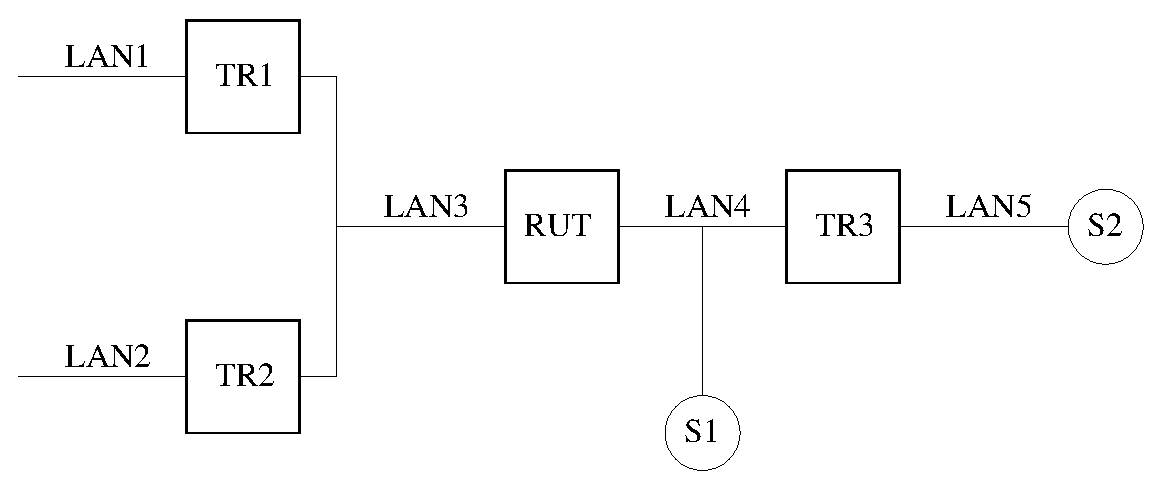
\includegraphics[scale=0.8]{figs/pim_test_4_3_receiving_sg_join_prune_messages}
    \caption{Receiving (S,G) Join/Prune messages test setup}
    \label{fig:receiving_sg_join_prune_messages}
  \end{center}
\end{figure}

\para{Procedure:}

\subpara{Part A: Receiving (S,G) Join messages at the first-hop router.}

\begin{enumerate}

  \item Configure the RUT as the RP. Start the RUT and TR1. If
  necessary, wait until the RP-set in the RUT and TR1 converges.

  \item Start observing the downstream (S,G) per-interface state
  machine at the RUT.

  \item Compose an (S,G) Join message at TR1 with the source address set
  to the address of S1, and send it to the RUT.
  The \verb=J/P_HoldTime= of the message should be set to its default
  value ({\PimsmJPHoldTime}).

  \item Start S1, and observe the data packets transmitted by the RUT on
  LAN3.

  \item Wait until the downstream (S,G) per-interface state in the RUT
  expires.

  \item Observe the data packets transmitted by the RUT on LAN3.

  \item Stop S1.

\end{enumerate}

\subpara{Part B: Receiving (S,G) Prune messages at the first-hop router.}

\begin{enumerate}

  \item Configure the RUT as the RP. Start the RUT and TR1. If
  necessary, wait until the RP-set in the RUT and TR1 converges.

  \item Start observing the downstream (S,G) per-interface state
  machine at the RUT.

  \item Compose an (S,G) Prune message at TR1 with the source address set
  to the address of S1, and send it to the RUT.
  The \verb=J/P_HoldTime= of the message should be set to its default
  value ({\PimsmJPHoldTime}).

  \item Compose an (S,G) Join message at TR1 with the source address set
  to the address of S1, and send it to the RUT.
  The \verb=J/P_HoldTime= of the message should be set to its default
  value ({\PimsmJPHoldTime}).

  \item Start S1, and observe the data packets transmitted by the RUT on
  LAN3.

  \item Compose an (S,G) Prune message at TR1 with the source address set
  to the address of S1, and send it to the RUT.

  \item Observe the messages and data packets transmitted by the RUT on
  LAN3.

  \item Stop S1.

\end{enumerate}

\subpara{Part C: Receiving (S,G) Join messages at non-first-hop router.}

\begin{enumerate}

  \item Configure TR3 as the RP. Start the RUT, TR1, and TR3. If
  necessary, wait until the RP-set in the RUT, TR1, and TR3
  converges.

  \item Start observing the downstream (S,G) per-interface state
  machine at the RUT.

  \item Compose an (S,G) Join message at TR1 with the source address set
  to the address of S2, and send it to the RUT.
  The \verb=J/P_HoldTime= of the message should be set to its default
  value ({\PimsmJPHoldTime}).

  \item Observe the messages transmitted by the RUT on LAN4.

  \item Start S2, and observe the data packets transmitted by the RUT on
  LAN3.

  \item Wait until the downstream (S,G) per-interface state in the RUT
  expires.

  \item Observe the data packets transmitted by the RUT on LAN3.

  \item Stop S2.

\end{enumerate}

\subpara{Part D: Receiving (S,G) Prune messages at non-first-hop router.}

\begin{enumerate}

  \item Configure TR3 as the RP. Start the RUT, TR1, and TR3. If
  necessary, wait until the RP-set in the RUT, TR1, and TR3
  converges.

  \item Start observing the downstream (S,G) per-interface state
  machine at the RUT.

  \item Compose an (S,G) Prune message at TR1 with the source address set
  to the address of S2, and send it to the RUT.
  The \verb=J/P_HoldTime= of the message should be set to its default
  value ({\PimsmJPHoldTime}).

  \item Compose an (S,G) Join message at TR1 with the source address set
  to the address of S2, and send it to the RUT.
  The \verb=J/P_HoldTime= of the message should be set to its default
  value ({\PimsmJPHoldTime}).

  \item Observe the messages transmitted by the RUT on LAN4.

  \item Start S2, and observe the data packets transmitted by the RUT on
  LAN3.

  \item Compose an (S,G) Prune message at TR1 with the source address set
  to the address of S2, and send it to the RUT.

  \item Observe the messages transmitted by the RUT on LAN3 and LAN4,
  and the data packets transmitted by the RUT on LAN3.

  \item Stop S2.

\end{enumerate}

\subpara{Part E: Receiving (S,G) Prune messages on a LAN.}

This part is same as Part D, except that in Step 1 we start TR2 as well.

\subpara{Part F: Receiving (S,G) Join and Prune messages on a LAN.}

This part is same as Part E, except that in Step 2 we compose and send
same (S,G) Join message from TR2 as well.

\para{Observable Results:}

\subpara{Part A:}

\begin{itemize}

  \item After the (S,G) Join message is received by the RUT, it
  should create the appropriate (S,G) multicast routing entry for
  that source and group, and the interface toward LAN3 should be in Join state
  and added to the set of outgoing interface for that entry:

\begin{verbatim}
Xorp> show pim join 
Group           Source          RP              Flags
224.0.1.20      10.3.0.2        10.3.0.1        SG DirectlyConnectedS 
    Upstream interface (S):   dc1
    Upstream interface (RP):  register_vif
    Upstream MRIB next hop (RP): UNKNOWN
    Upstream MRIB next hop (S):  UNKNOWN
    Upstream RPF'(*,G):       UNKNOWN
    Upstream RPF'(S,G):       UNKNOWN
    Upstream RPF'(S,G,rpt):   UNKNOWN
    Upstream state:           Joined 
    Register state:           RegisterNoinfo RegisterNotCouldRegister 
    Join timer:               51
    Local include:            ..............
    Local exclude:            ..............
    Local include WC:         ..............
    Local include SG:         ..............
    Local exclude SG:         ..............
    Joins RP:                 ..............
    Joins WC:                 ..............
    Joins SG:                 ......O.......
    Prunes SG_RPT:            ..............
    Join state:               ......O.......
    Prune state:              ..............
    Prune pending state:      ..............
    I am assert winner state: ..............
    I am assert loser state:  ..............
    Assert winner WC:         ..............
    Assert winner SG:         ..............
    Assert lost WC:           ..............
    Could assert SG:          ..............
    I am DR:                  .....OO.......
    Immediate olist RP:       ..............
    Immediate olist WC:       ..............
    Immediate olist SG:       ......O.......
    Inherited olist SG:       ......O.......
    Inherited olist SG_RPT:   ..............
    PIM include WC:           ..............
\end{verbatim}

  \item After S1 is started, the multicast data packets should be
  forwarded by the RUT on LAN3. In addition, the SPT flag for the
  entry should be set:

\begin{verbatim}
Xorp> show pim join 
Group           Source          RP              Flags
224.0.1.20      10.3.0.2        10.3.0.1        SG SPT DirectlyConnectedS 
    Upstream interface (S):   dc1
    Upstream interface (RP):  register_vif
    Upstream MRIB next hop (RP): UNKNOWN
    Upstream MRIB next hop (S):  UNKNOWN
    Upstream RPF'(*,G):       UNKNOWN
    Upstream RPF'(S,G):       UNKNOWN
    Upstream RPF'(S,G,rpt):   UNKNOWN
    Upstream state:           Joined 
    Register state:           RegisterNoinfo RegisterNotCouldRegister 
    Join timer:               19
    Local include:            ..............
    Local exclude:            ..............
    Local include WC:         ..............
    Local include SG:         ..............
    Local exclude SG:         ..............
    Joins RP:                 ..............
    Joins WC:                 ..............
    Joins SG:                 ......O.......
    Prunes SG_RPT:            ..............
    Join state:               ......O.......
    Prune state:              ..............
    Prune pending state:      ..............
    I am assert winner state: ..............
    I am assert loser state:  ..............
    Assert winner WC:         ..............
    Assert winner SG:         ..............
    Assert lost WC:           ..............
    Could assert SG:          ......O.......
    I am DR:                  .....OO.......
    Immediate olist RP:       ..............
    Immediate olist WC:       ..............
    Immediate olist SG:       ......O.......
    Inherited olist SG:       ......O.......
    Inherited olist SG_RPT:   ..............
    PIM include WC:           ..............
\end{verbatim}

  \item After \verb=J/P_HoldTime= ({\PimsmJPHoldTime}),
  the (S,G) state machine for the interface that connects the RUT to
  LAN3 should timeout and transition to NoInfo state.
  As a result of that transition, no multicast packets should be
  forwarded by the RUT on LAN3.
  However, the (S,G) state itself should not be removed yet, because the
  directly-connected sender is still active:

\begin{verbatim}
Xorp> show pim join 
Group           Source          RP              Flags
224.0.1.20      10.3.0.2        10.3.0.1        SG DirectlyConnectedS 
    Upstream interface (S):   dc1
    Upstream interface (RP):  register_vif
    Upstream MRIB next hop (RP): UNKNOWN
    Upstream MRIB next hop (S):  UNKNOWN
    Upstream RPF'(*,G):       UNKNOWN
    Upstream RPF'(S,G):       UNKNOWN
    Upstream RPF'(S,G,rpt):   UNKNOWN
    Upstream state:           NotJoined 
    Register state:           RegisterNoinfo RegisterNotCouldRegister 
    Join timer:               -1
    Local include:            ..............
    Local exclude:            ..............
    Local include WC:         ..............
    Local include SG:         ..............
    Local exclude SG:         ..............
    Joins RP:                 ..............
    Joins WC:                 ..............
    Joins SG:        B         ..............
    Prunes SG_RPT:            ..............
    Join state:               ..............
    Prune state:              ..............
    Prune pending state:      ..............
    I am assert winner state: ..............
    I am assert loser state:  ..............
    Assert winner WC:         ..............
    Assert winner SG:         ..............
    Assert lost WC:           ..............
    Could assert SG:          ..............
    I am DR:                  .....OO.......
    Immediate olist RP:       ..............
    Immediate olist WC:       ..............
    Immediate olist SG:       ..............
    Inherited olist SG:       ..............
    Inherited olist SG_RPT:   ..............
    PIM include WC:           ..............
\end{verbatim}

 \item After the sender is stopped, and after it has been inactive
  for \verb=Keepalive_Period= ({\PimsmKeepalivePeriod}), the (S,G) state
  should expire.

\end{itemize}

\subpara{Part B:}

\begin{itemize}

  \item After the (S,G) Prune message is received by the RUT,
  the (S,G) state machine for the interface that connects the RUT to
  LAN3 should continue to stay in the NoInfo state (\ie no (S,G) multicast
  routing entry should be created).

  \item After that, the results until after S1 is started should be same as in
  Part A.

  \item After the (S,G) Prune message is received by the RUT,
  the (S,G) state machine for the interface that connects the RUT to
  LAN3 should transition to NoInfo state.
  As a result of that transition no multicast packets should be
  forwarded by the RUT on LAN3.
  However, the (S,G) state itself should not be removed yet, because the
  directly-connected sender is still active (see Part A).

 \item After the sender is stopped, and after it has been inactive
  for \verb=Keepalive_Period= ({\PimsmKeepalivePeriod}), the (S,G) state
  should expire.

\end{itemize}

\subpara{Part C:}

\begin{itemize}

  \item After the (S,G) Join message is received by the RUT, it
  should create the appropriate (S,G) multicast routing entry for
  that source and group, and the interface toward LAN3 should be in Join state
  and added to the set of outgoing interface for that entry:

\begin{verbatim}
Xorp> show pim join 
Group           Source          RP              Flags
224.0.1.20      10.4.0.2        10.4.0.1        SG   
    Upstream interface (S):   dc1
    Upstream interface (RP):  dc1
    Upstream MRIB next hop (RP): 10.3.0.2
    Upstream MRIB next hop (S):  10.3.0.2
    Upstream RPF'(*,G):       UNKNOWN
    Upstream RPF'(S,G):       10.3.0.2
    Upstream RPF'(S,G,rpt):   UNKNOWN
    Upstream state:           Joined 
    Register state:           
    Join timer:               47
    Local include:            ..............
    Local exclude:            ..............
    Local include WC:         ..............
    Local include SG:         ..............
    Local exclude SG:         ..............
    Joins RP:                 ..............
    Joins WC:                 ..............
    Joins SG:                 ......O.......
    Prunes SG_RPT:            ..............
    Join state:               ......O.......
    Prune state:              ..............
    Prune pending state:      ..............
    I am assert winner state: ..............
    I am assert loser state:  ..............
    Assert winner WC:         ..............
    Assert winner SG:         ..............
    Assert lost WC:           ..............
    Could assert SG:          ..............
    I am DR:                  ......O.......
    Immediate olist RP:       ..............
    Immediate olist WC:       ..............
    Immediate olist SG:       ......O.......
    Inherited olist SG:       ......O.......
    Inherited olist SG_RPT:   ..............
    PIM include WC:           ..............
\end{verbatim}

  Further, the RUT itself should originate an (S,G) Join message
  toward the source (S2).

  \item After S2 is started, the multicast data packets forwarded by TR3
  on LAN4 should be forwarded by the RUT on LAN3. Further, the SPT-bit for the
  entry should be set:

\begin{verbatim}
Xorp> show pim join 
Group           Source          RP              Flags
224.0.1.20      10.4.0.2        10.4.0.1        SG SPT 
    Upstream interface (S):   dc1
    Upstream interface (RP):  dc1
    Upstream MRIB next hop (RP): 10.3.0.2
    Upstream MRIB next hop (S):  10.3.0.2
    Upstream RPF'(*,G):       UNKNOWN
    Upstream RPF'(S,G):       10.3.0.2
    Upstream RPF'(S,G,rpt):   UNKNOWN
    Upstream state:           Joined 
    Register state:           
    Join timer:               19
    Local include:            ..............
    Local exclude:            ..............
    Local include WC:         ..............
    Local include SG:         ..............
    Local exclude SG:         ..............
    Joins RP:                 ..............
    Joins WC:                 ..............
    Joins SG:                 ......O.......
    Prunes SG_RPT:            ..............
    Join state:               ......O.......
    Prune state:              ..............
    Prune pending state:      ..............
    I am assert winner state: ..............
    I am assert loser state:  ..............
    Assert winner WC:         ..............
    Assert winner SG:         ..............
    Assert lost WC:           ..............
    Could assert SG:          ......O.......
    I am DR:                  ......O.......
    Immediate olist RP:       ..............
    Immediate olist WC:       ..............
    Immediate olist SG:       ......O.......
    Inherited olist SG:       ......O.......
    Inherited olist SG_RPT:   ..............
    PIM include WC:           ..............
\end{verbatim}

  \item After \verb=J/P_HoldTime= ({\PimsmJPHoldTime}),
  the (S,G) state machine for the interface that connects the RUT to
  LAN3 should timeout and transition to NoInfo state
  As a result of that transition, the RUT should send (S,G) Prune
  message toward the source (S2), and no multicast packets should be
  forwarded by the RUT on LAN3.
  Note that if the implementation does not remove (S,G) states that
  have the Keepalive Timer running, the entry may not be removed yet:

\begin{verbatim}
Xorp> show pim join 
Group           Source          RP              Flags
224.0.1.20      10.4.0.2        10.4.0.1        SG   
    Upstream interface (S):   dc1
    Upstream interface (RP):  dc1
    Upstream MRIB next hop (RP): 10.3.0.2
    Upstream MRIB next hop (S):  10.3.0.2
    Upstream RPF'(*,G):       UNKNOWN
    Upstream RPF'(S,G):       10.3.0.2
    Upstream RPF'(S,G,rpt):   UNKNOWN
    Upstream state:           NotJoined 
    Register state:           
    Join timer:               -1
    Local include:            ..............
    Local exclude:            ..............
    Local include WC:         ..............
    Local include SG:         ..............
    Local exclude SG:         ..............
    Joins RP:                 ..............
    Joins WC:                 ..............
    Joins SG:                 ..............
    Prunes SG_RPT:            ..............
    Join state:               ..............
    Prune state:              ..............
    Prune pending state:      ..............
    I am assert winner state: ..............
    I am assert loser state:  ..............
    Assert winner WC:         ..............
    Assert winner SG:         ..............
    Assert lost WC:           ..............
    Could assert SG:          ..............
    I am DR:                  ......O.......
    Immediate olist RP:       ..............
    Immediate olist WC:       ..............
    Immediate olist SG:       ..............
    Inherited olist SG:       ..............
    Inherited olist SG_RPT:   ..............
    PIM include WC:           ..............
\end{verbatim}

 \item After the sender is stopped, and after it has been inactive
  for \verb=Keepalive_Period= ({\PimsmKeepalivePeriod}), the (S,G) state
  should expire if it was not removed earlier.

\end{itemize}

\subpara{Part D:}

\begin{itemize}

  \item After the (S,G) Prune message is received by the RUT,
  the (S,G) state machine for the interface that connects the RUT to
  LAN3 should continue to stay in the NoInfo state (\ie no (S,G) multicast
  routing entry should be created).

  \item After that, the results until after S2 is started should be same as in
  Part C.

  \item After the (S,G) Prune message from TR1 is received by the RUT,
  the (S,G) state machine for the interface that connects the RUT to
  LAN3 should transition to NoInfo state. This may or may not remove
  the (S,G) state itself (see the observable results in Part C).
  As a result of that transition, the RUT should send (S,G) Prune
  message toward the source (S2), and no multicast packets should be
  forwarded by the RUT on LAN3. Note that because the RUT has only one
  PIM neighbor on LAN3, it does not need to send (S,G) PruneEcho on
  LAN3.

\end{itemize}

\subpara{Part E:}

\begin{itemize}

  \item The results until after S2 is started should be same as in
  Part C and D.

  \item After the (S,G) Prune message from TR1 is received by the RUT,
  the (S,G) state machine for the interface that connects the RUT to
  LAN3 should transition to PrunePending state (the reason that it does
  not transit to NoInfo instead is because the RUT has more than one PIM
  neighbors on that interface).
  After \verb=J/P_Override_Interval(I)= (\PimsmJPOverrideIntervalI),
  the PrunePending timer on that interface should expire, and the
  (S,G) state machine for the interface should send (S,G) PruneEcho
  on LAN3 and transit to NoInfo
  state. This may or may not remove the (S,G) state itself (see the observable
  results in Part C).
  As a result of that transition, the RUT should send (S,G) Prune
  message toward the source (S2), and no multicast packets should be
  forwarded by the RUT on LAN3.

\end{itemize}

\subpara{Part F:}

\begin{itemize}

  \item The results until after S2 is started should be same as in
  Part C, D, and E.

  \item After the (S,G) Prune message from TR1 is received by the RUT,
  the (S,G) state machine for the interface that connects the RUT to
  LAN3 should transition to PrunePending state (the reason that it does
  not transit to NoInfo instead is because the RUT has more than one PIM
  neighbors on that interface).
  Assuming that TR2 has (S,G) multicast routing entry in Joined state
  for the source it had originated (S,G) Join message earlier, then after
  very short random interval \verb=t_override= ({\PimsmTOverride}) TR2
  should send another (S,G) Join message to the RUT.
  After the RUT receives that (S,G) Join message from TR2,
  the (S,G) state machine for the interface that connects the RUT to
  LAN3 should transition back to Join state.
  As a result of that transition, the RUT should not send (S,G) Prune
  message toward the source (S2), and the multicast packets should continue
  to be forwarded by the RUT on LAN3.

\end{itemize}

\para{Possible Problems:}
None.

%%%%%%%%%%%%%%%%%%%%%%%%%%%%%%%%%%%%%%%%%%%
\newpage
\section{Receiving (S,G,rpt) Join/Prune Messages}

\para{Purpose:}
Verify that (S,G,rpt) Join/Prune messages are received and processed
properly.

\para{References:}
\begin{itemize}
  \item draft-ietf-pim-sm-v2-new-05 -- Section 4.5.4
\end{itemize}

\para{Discussion:}
When a PIM-SM router receives a PIM (S,G,rpt) Join/Prune message, the
per-interface (S,G,rpt) state-machine should be updated appropriately.
Typically, if an (S,G,rpt) Prune message is received, it should
remove the interface it was received on from the set of outgoing interfaces
for that source and group. If that set has just became empty, an (S,G,rpt)
Prune message should be sent toward the RP.
If an (S,G,rpt) Join message is received, typically the interface it was
received on should be removed from the list of pruned outgoing interfaces for
that source and group.

\para{Test Setup:}
Connect the RUT, TR1, TR2, TR3, S1, and S2 according to
Figure~\ref{fig:receiving_sg_rpt_join_prune_messages}~\footnote{Note that S1 is
used only when TR3 and S2 are not used, hence it is not necessary to have two
senders at same time.}.
Enable PIM-SM on the RUT, TR1, TR2, and TR3.
Configure S1 and S2 as senders for group 224.0.1.20~\footnote{Note that
currently TR3 and S2 are not used in the test scenarios described below.}.

\begin{figure}[htbp]
  \begin{center}
    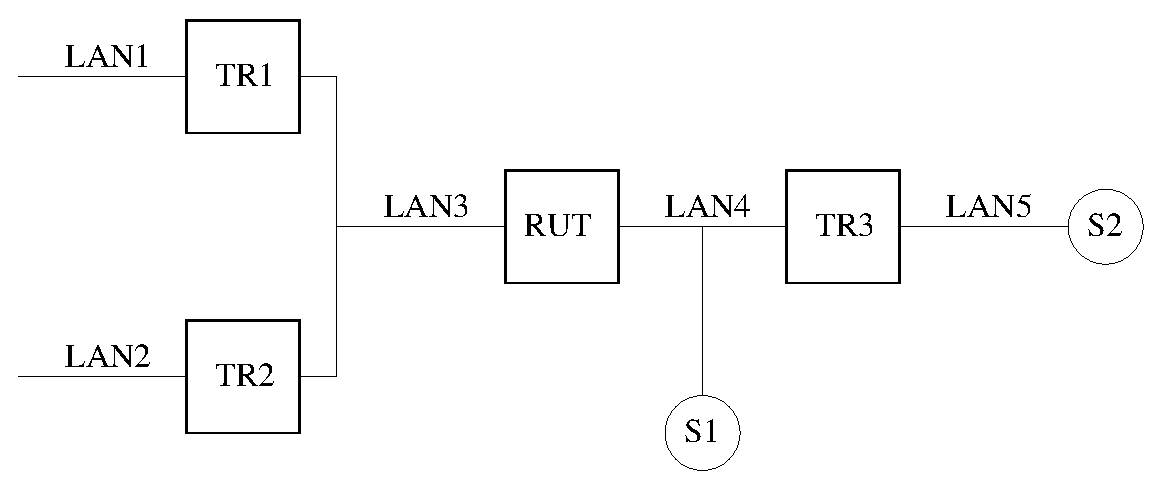
\includegraphics[scale=0.8]{figs/pim_test_4_4_receiving_sg_rpt_join_prune_messages}
    \caption{Receiving (S,G,rpt) Join/Prune messages test setup}
    \label{fig:receiving_sg_rpt_join_prune_messages}
  \end{center}
\end{figure}

\para{Procedure:}

\subpara{Part A: Receiving (S,G,rpt) Join messages at the first-hop router.}

\begin{enumerate}

  \item Configure the RUT as the RP. Start the RUT and TR1. If
  necessary, wait until the RP-set in the RUT and TR1 converges.

  \item Start observing the downstream (S,G,rpt) per-interface state
  machine at the RUT.

  \item Compose an (S,G,rpt) Join message at TR1 with the source address set
  to the address of S1, and send it to the RUT.
  The \verb=J/P_HoldTime= of the message should be set to its default
  value ({\PimsmJPHoldTime}).

  \item Observe the downstream (S,G,rpt) per-interface state in the RUT.

  \item Start S1, and observe the data packets transmitted by the RUT on
  LAN3.

\end{enumerate}

\subpara{Part B: Receiving (S,G,rpt) Prune messages at the first-hop router.}

\begin{enumerate}

  \item Configure the RUT as the RP. Start the RUT and TR1. If
  necessary, wait until the RP-set in the RUT and TR1 converges.

  \item Start observing the downstream (S,G,rpt) per-interface state
  machine at the RUT.

  \item Compose an (S,G,rpt) Prune message at TR1 with the source address set
  to the address of S1, and send it to the RUT.
  The \verb=J/P_HoldTime= of the message should be set to its default
  value ({\PimsmJPHoldTime}).

  \item Observe the downstream (S,G,rpt) per-interface state in the RUT
  for at least \verb=J/P_HoldTime= ({\PimsmJPHoldTime}).

\end{enumerate}

\subpara{Part C: Receiving (S,G,rpt) Prune and (S,G,rpt) Join messages at the
first-hop router.}

\begin{enumerate}

  \item Configure the RUT as the RP. Start the RUT and TR1. If
  necessary, wait until the RP-set in the RUT and TR1 converges.

  \item Start observing the downstream (S,G,rpt) per-interface state
  machine at the RUT.

  \item Compose an (S,G,rpt) Prune message at TR1 with the source address set
  to the address of S1, and send it to the RUT.
  The \verb=J/P_HoldTime= of the message should be set to its default
  value ({\PimsmJPHoldTime}).

  \item Observe the downstream (S,G,rpt) per-interface state in the RUT.

  \item Start S1, and observe the data packets transmitted by the RUT on
  LAN3.

  \item Compose an (S,G,rpt) Join message at TR1 with the source address set
  to the address of S1, and send it to the RUT.
  The \verb=J/P_HoldTime= of the message should be set to its default
  value ({\PimsmJPHoldTime}).

  \item Observe the downstream (S,G,rpt) per-interface state in the RUT.

  \item Stop S1.

\end{enumerate}

\subpara{Part D: Receiving (S,G,rpt) Prune and (*,G) Join messages at the
first-hop router.}

\begin{enumerate}

  \item Configure the RUT as the RP. Start the RUT and TR1. If
  necessary, wait until the RP-set in the RUT and TR1 converges.

  \item Start observing the downstream (S,G,rpt) per-interface state
  machine at the RUT.

  \item Compose an (S,G,rpt) Prune message at TR1 with the source address set
  to the address of S1, and send it to the RUT.
  The \verb=J/P_HoldTime= of the message should be set to its default
  value ({\PimsmJPHoldTime}).

  \item Observe the downstream (S,G,rpt) per-interface state in the RUT.

  \item Start S1, and observe the data packets transmitted by the RUT on
  LAN3.

  \item Compose an (*,G) Join message at TR1 with the source address set
  to the address of S1, and send it to the RUT.
  The \verb=J/P_HoldTime= of the message should be set to its default
  value ({\PimsmJPHoldTime}).

  \item Observe the downstream (S,G,rpt) per-interface state in the RUT.

  \item Compose a message at TR1 that contains (*,G) Join with the RP
  address set to the address of the RUT, and (S,G,rpt) Prune with the source
  address set to the address of S1, and send it to the RUT.
  The \verb=J/P_HoldTime= of the message should be set to its default
  value ({\PimsmJPHoldTime}).

  \item Observe the downstream (S,G,rpt) per-interface state in the RUT.

  \item Stop S1.

\end{enumerate}

\para{Observable Results:}

\subpara{Part A:}

\begin{itemize}

  \item After the (S,G,rpt) Join message is received by the RUT,
  the (S,G,rpt) state machine for the interface that connects the RUT to
  LAN3 should continue to stay in the NoInfo state (\ie no (S,G,rpt) multicast
  routing entry should be created).

  \item After S1 is started, no multicast packets should be
  forwarded by the RUT on LAN3.

\end{itemize}

\subpara{Part B:}

\begin{itemize}

  \item After the (S,G,rpt) Prune message is received by the RUT,
  the (S,G,rpt) state machine for the interface that connects the RUT to
  LAN3 should transition to PrunePending state. The state machine should
  remain in that state for \verb=J/P_Override_Interval(I)=
  ({\PimsmJPOverrideIntervalI}). After that it should transition to Prune
  state:

\begin{verbatim}
Xorp> show pim join 
Group           Source          RP              Flags
224.0.1.20      10.3.0.2        10.3.0.1        SG_RPT DirectlyConnectedS 
    Upstream interface (S):   dc1
    Upstream interface (RP):  register_vif
    Upstream MRIB next hop (RP): UNKNOWN
    Upstream MRIB next hop (S):  UNKNOWN
    Upstream RPF'(S,G,rpt):   UNKNOWN
    Upstream state:           NotJoined RptNotJoined 
    Override timer:           -1
    Local include:            ................
    Local exclude:            ................
    Local include WC:         ................
    Local include SG:         ................
    Local exclude SG:         ................
    Joins RP:                 ................
    Joins WC:                 ................
    Joins SG:                 ................
    Prunes SG_RPT:            ......O.........
    Join state:               ................
    Prune state:              ......O.........
    Prune pending state:      ................
    Prune tmp state:          ................
    Prune pending tmp state:  ................
    I am assert winner state: ................
    I am assert loser state:  ................
    Assert winner WC:         ................
    Assert winner SG:         ................
    Assert lost WC:           ................
    Assert lost SG:           ................
    Assert lost SG_RPT:       ................
    Assert tracking WC:       ................
    Assert tracking SG:       ................
    Could assert WC:          ................
    Could assert SG:          ................
    I am DR:                  .....OO.........
    Immediate olist RP:       ................
    Immediate olist WC:       ................
    Immediate olist SG:       ................
    Inherited olist SG:       ................
    Inherited olist SG_RPT:   ................
    PIM include WC:           ................
    PIM include SG:           ................
    PIM exclude SG:           ................
\end{verbatim}

  The Expiry Timer for the interface that connects the RUT to LAN3
  should expire after \verb=J/P_HoldTime= ({\PimsmJPHoldTime}).
  After it expires, the state machine for that interface should transition to
  NoInfo state, and the (S,G,rpt) state itself should be removed.

\end{itemize}

\subpara{Part C:}

\begin{itemize}

  \item Until after the (S,G,rpt) Prune message is received by the RUT, the
  results should be same as in Part B.

  \item After the (S,G,rpt) Join message is received by the RUT,
  the (S,G,rpt) state machine for the interface that connects the RUT to
  LAN3 should transition to NoInfo state, and the (S,G,rpt) state itself
  should be removed.

  \item At all time after S1 is started, no multicast packets should be
  forwarded by the RUT on LAN3.

\end{itemize}

\subpara{Part D:}

\begin{itemize}

  \item Until after the (S,G,rpt) Prune message is received by the RUT, the
  results should be same as in Part B and Part C.

  \item After S1 is started, no multicast packets should be
  forwarded by the RUT on LAN3.

  \item After the (*,G) Join message is received by the RUT,
  the (S,G,rpt) state machine for the interface that connects the RUT to
  LAN3 should transition to NoInfo state, and the (S,G,rpt) state itself
  should be removed. However, the RUT should have created an (*,G) state.
  The (*,G) state machine for the interface that connects the RUT to
  LAN3 should be in Join state (note that after S1 is started, the router
  would have (S,G) routing state as well because of the directly-connected
  source):

\begin{verbatim}
Xorp> show pim join 
Group           Source          RP              Flags
224.0.1.20      0.0.0.0         10.3.0.1        WC   
    Upstream interface (RP):  register_vif
    Upstream MRIB next hop (RP): UNKNOWN
    Upstream RPF'(*,G):       UNKNOWN
    Upstream state:           Joined 
    Join timer:               51
    Local include:            ................
    Local exclude:            ................
    Local include WC:         ................
    Local include SG:         ................
    Local exclude SG:         ................
    Joins RP:                 ................
    Joins WC:                 ......O.........
    Joins SG:                 ................
    Prunes SG_RPT:            ................
    Join state:               ......O.........
    Prune state:              ................
    Prune pending state:      ................
    Prune tmp state:          ................
    Prune pending tmp state:  ................
    I am assert winner state: ................
    I am assert loser state:  ................
    Assert winner WC:         ................
    Assert winner SG:         ................
    Assert lost WC:           ................
    Assert lost SG:           ................
    Assert lost SG_RPT:       ................
    Assert tracking WC:       ......O........O
    Assert tracking SG:       ................
    Could assert WC:          ......O.........
    Could assert SG:          ................
    I am DR:                  .....OO.........
    Immediate olist RP:       ................
    Immediate olist WC:       ......O.........
    Immediate olist SG:       ................
    Inherited olist SG:       ................
    Inherited olist SG_RPT:   ................
    PIM include WC:           ................
    PIM include SG:           ................
    PIM exclude SG:           ................
224.0.1.20      10.3.0.2        10.3.0.1        SG DirectlyConnectedS 
    Upstream interface (S):   dc1
    Upstream interface (RP):  register_vif
    Upstream MRIB next hop (RP): UNKNOWN
    Upstream MRIB next hop (S):  UNKNOWN
    Upstream RPF'(S,G):       UNKNOWN
    Upstream state:           Joined 
    Register state:           RegisterNoinfo RegisterNotCouldRegister 
    Join timer:               51
    Local include:            ................
    Local exclude:            ................
    Local include WC:         ................
    Local include SG:         ................
    Local exclude SG:         ................
    Joins RP:                 ................
    Joins WC:                 ......O.........
    Joins SG:                 ................
    Prunes SG_RPT:            ................
    Join state:               ................
    Prune state:              ................
    Prune pending state:      ................
    Prune tmp state:          ................
    Prune pending tmp state:  ................
    I am assert winner state: ................
    I am assert loser state:  ................
    Assert winner WC:         ................
    Assert winner SG:         ................
    Assert lost WC:           ................
    Assert lost SG:           ................
    Assert lost SG_RPT:       ................
    Assert tracking WC:       ......O........O
    Assert tracking SG:       .....OO........O
    Could assert WC:          ......O.........
    Could assert SG:          ................
    I am DR:                  .....OO.........
    Immediate olist RP:       ................
    Immediate olist WC:       ......O.........
    Immediate olist SG:       ................
    Inherited olist SG:       ......O.........
    Inherited olist SG_RPT:   ................
    PIM include WC:           ................
    PIM include SG:           ................
    PIM exclude SG:           ................
\end{verbatim}

  The multicast packets from S1 should be forwarded by the RUT on LAN3.

  \item After the message with the (*,G) Join and (S,G,rpt) Prune is received
  by the RUT, the (*,G) state machine for the interface that connects the RUT
  to LAN3 should remain in Join state, but
  the (S,G,rpt) state machine for the interface that connects the RUT to
  LAN3 should transition to Prune state:

\begin{verbatim}
Xorp> show pim join 
Group           Source          RP              Flags
224.0.1.20      0.0.0.0         10.3.0.1        WC   
    Upstream interface (RP):  register_vif
    Upstream MRIB next hop (RP): UNKNOWN
    Upstream RPF'(*,G):       UNKNOWN
    Upstream state:           Joined 
    Join timer:               28
    Local include:            ................
    Local exclude:            ................
    Local include WC:         ................
    Local include SG:         ................
    Local exclude SG:         ................
    Joins RP:                 ................
    Joins WC:                 ......O.........
    Joins SG:                 ................
    Prunes SG_RPT:            ................
    Join state:               ......O.........
    Prune state:              ................
    Prune pending state:      ................
    Prune tmp state:          ................
    Prune pending tmp state:  ................
    I am assert winner state: ................
    I am assert loser state:  ................
    Assert winner WC:         ................
    Assert winner SG:         ................
    Assert lost WC:           ................
    Assert lost SG:           ................
    Assert lost SG_RPT:       ................
    Assert tracking WC:       ......O........O
    Assert tracking SG:       ................
    Could assert WC:          ......O.........
    Could assert SG:          ................
    I am DR:                  .....OO.........
    Immediate olist RP:       ................
    Immediate olist WC:       ......O.........
    Immediate olist SG:       ................
    Inherited olist SG:       ................
    Inherited olist SG_RPT:   ................
    PIM include WC:           ................
    PIM include SG:           ................
    PIM exclude SG:           ................
224.0.1.20      10.3.0.2        10.3.0.1        SG_RPT DirectlyConnectedS 
    Upstream interface (S):   dc1
    Upstream interface (RP):  register_vif
    Upstream MRIB next hop (RP): UNKNOWN
    Upstream MRIB next hop (S):  UNKNOWN
    Upstream RPF'(S,G,rpt):   UNKNOWN
    Upstream state:           NotJoined Pruned 
    Override timer:           -1
    Local include:            ................
    Local exclude:            ................
    Local include WC:         ................
    Local include SG:         ................
    Local exclude SG:         ................
    Joins RP:                 ................
    Joins WC:                 ......O.........
    Joins SG:                 ................
    Prunes SG_RPT:            ......O.........
    Join state:               ................
    Prune state:              ......O.........
    Prune pending state:      ................
    Prune tmp state:          ................
    Prune pending tmp state:  ................
    I am assert winner state: ................
    I am assert loser state:  ................
    Assert winner WC:         ................
    Assert winner SG:         ................
    Assert lost WC:           ................
    Assert lost SG:           ................
    Assert lost SG_RPT:       ................
    Assert tracking WC:       ......O........O
    Assert tracking SG:       ................
    Could assert WC:          ......O.........
    Could assert SG:          ................
    I am DR:                  .....OO.........
    Immediate olist RP:       ................
    Immediate olist WC:       ......O.........
    Immediate olist SG:       ................
    Inherited olist SG:       ................
    Inherited olist SG_RPT:   ................
    PIM include WC:           ................
    PIM include SG:           ................
    PIM exclude SG:           ................
224.0.1.20      10.3.0.2        10.3.0.1        SG DirectlyConnectedS 
    Upstream interface (S):   dc1
    Upstream interface (RP):  register_vif
    Upstream MRIB next hop (RP): UNKNOWN
    Upstream MRIB next hop (S):  UNKNOWN
    Upstream RPF'(S,G):       UNKNOWN
    Upstream state:           NotJoined 
    Register state:           RegisterNoinfo RegisterNotCouldRegister 
    Join timer:               -1
    Local include:            ................
    Local exclude:            ................
    Local include WC:         ................
    Local include SG:         ................
    Local exclude SG:         ................
    Joins RP:                 ................
    Joins WC:                 ......O.........
    Joins SG:                 ................
    Prunes SG_RPT:            ................
    Join state:               ................
    Prune state:              ................
    Prune pending state:      ................
    Prune tmp state:          ................
    Prune pending tmp state:  ................
    I am assert winner state: ................
    I am assert loser state:  ................
    Assert winner WC:         ................
    Assert winner SG:         ................
    Assert lost WC:           ................
    Assert lost SG:           ................
    Assert lost SG_RPT:       ................
    Assert tracking WC:       ......O........O
    Assert tracking SG:       ...............O
    Could assert WC:          ......O.........
    Could assert SG:          ................
    I am DR:                  .....OO.........
    Immediate olist RP:       ................
    Immediate olist WC:       ......O.........
    Immediate olist SG:       ................
    Inherited olist SG:       ................
    Inherited olist SG_RPT:   ................
    PIM include WC:           ................
    PIM include SG:           ................
    PIM exclude SG:           ................
\end{verbatim}

  The multicast packets from S1 should stop being forwarded by the RUT on
  LAN3.

\end{itemize}

\para{Possible Problems:}
None.

%%%%%%%%%%%%%%%%%%%%%%%%%%%%%%%%%%%%%%%%%%%
\newpage
\section{Sending (*,*,RP) Join/Prune Messages}

\para{Purpose:}
Verify that (*,*,RP) Join/Prune messages are sent properly.

\para{References:}
\begin{itemize}
  \item draft-ietf-pim-sm-v2-new-05 -- Section 4.5.5
\end{itemize}

\para{Discussion:}
If a router receives an (*,*,RP) Join/Prune message, it may need to propagate
it toward the RP. A router should monitor its upstream interface for messages
from other routers on that subnet, and if it sees an (*,*,RP) Join to the
correct upstream neighbor, it should suporess its own (*,*,RP) Join message.
If it sees an (*,*,RP) Prune, it should override that prune by sending an
(*,*,RP) Join almost immediately. If a router sees the Generation ID of the
correct upstream neighbor change, the router should refresh the state by
sending an (*,*,RP) Join almost immediately. In addition, if the MRIB changes
to indicate that the next hop towards the RP has changed, the router should
send an (*,*,RP) towards the old next hop, and send an (*,*,RP) towards the
next next hop router.

\para{Test Setup:}
Connect the RUT, TR1, TR2, TR3, TR4, and S1 according to
Figure~\ref{fig:pim_test_4_5_sending_rp_join_prune_messages}.
In all tests, configure the RUT such that the next-hop route toward LAN6 is
TR4, unless stated otherwise.

\begin{figure}[htbp]
  \begin{center}
    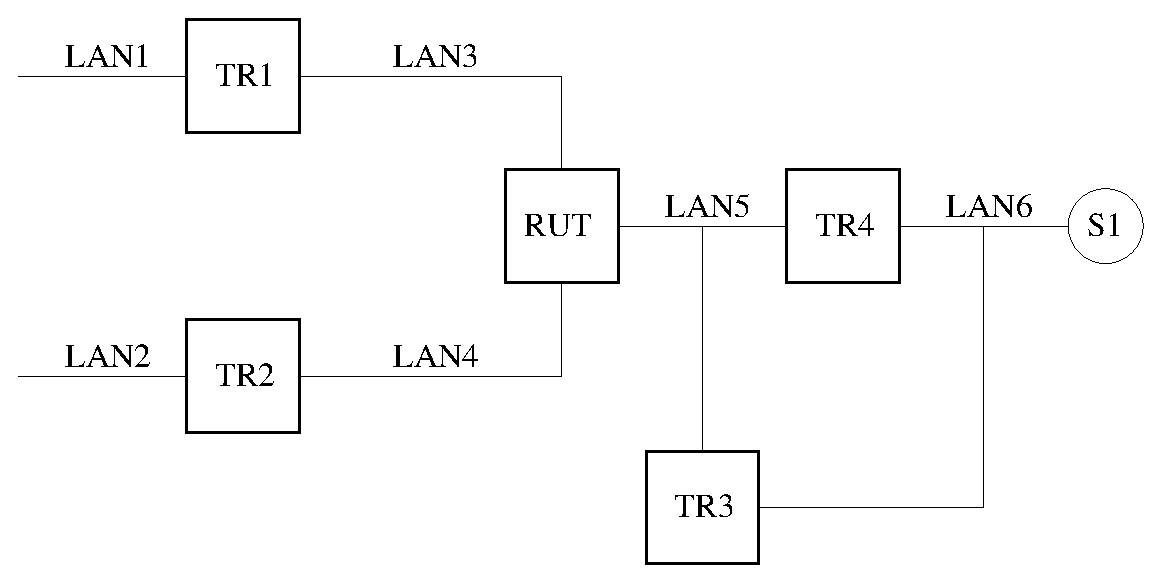
\includegraphics[scale=0.8]{figs/pim_test_4_5_sending_rp_join_prune_messages}
    \caption{Sending (*,*,RP) Join/Prune Messages test setup}
    \label{fig:pim_test_4_5_sending_rp_join_prune_messages}
  \end{center}
\end{figure}

\para{Procedure:}

\subpara{Part A: JoinDesired(*,*,RP) $\Longrightarrow$ True/False transaction.}

\begin{enumerate}

  \item Configure TR4 as the RP. Start the RUT, TR1, TR2, and TR4. If
  necessary, wait until the RP-set in the RUT, TR1, TR2, and TR4
  converges.

  \item Start observing the (*,*,RP) Join/Prune messages transmitted by the
  RUT on LAN5.

  \item Compose an (*,*,RP) Join message at TR1 with the RP address set to the
  address of TR4, and send it to the RUT. 
  The \verb=J/P_HoldTime= of the message should be set to its default
  value ({\PimsmJPHoldTime}).

  \item Compose an (*,*,RP) Prune message at TR1 with the RP address set to the
  address of TR4, and send it to the RUT. 
  The \verb=J/P_HoldTime= of the message should be set to its default
  value ({\PimsmJPHoldTime}).

  \item Compose an (*,*,RP) Join message at TR1 with the RP address set to the
  address of TR4, and send it to the RUT. 
  The \verb=J/P_HoldTime= of the message should be set to its default
  value ({\PimsmJPHoldTime}).

  \item Compose an (*,*,RP) Join message at TR2 with the RP address set to the
  address of TR4, and send it to the RUT. 
  The \verb=J/P_HoldTime= of the message should be set to its default
  value ({\PimsmJPHoldTime}).

  \item Compose an (*,*,RP) Prune message at TR2 with the RP address set to the
  address of TR4, and send it to the RUT. 
  The \verb=J/P_HoldTime= of the message should be set to its default
  value ({\PimsmJPHoldTime}).

\end{enumerate}

\subpara{Part B: (*,*,RP) Join Timer expiration.}

\begin{enumerate}

  \item Configure TR4 as the RP. Start the RUT, TR1, and TR4. If
  necessary, wait until the RP-set in the RUT, TR1, and TR4
  converges.

  \item Start observing the (*,*,RP) Join/Prune messages transmitted by the
  RUT on LAN5.

  \item Compose an (*,*,RP) Join message at TR1 with the RP address set to the
  address of TR4, and send it to the RUT. 
  The \verb=J/P_HoldTime= of the message should be set to its default
  value ({\PimsmJPHoldTime}).

  \item Keep observing the (*,*,RP) Join/Prune messages transmitted by the
  RUT on LAN5 for at least \verb=J/P_HoldTime= ({\PimsmJPHoldTime}).

\end{enumerate}

\subpara{Part C: See (*,*,RP) Join message to MRIB.next\_hop(RP).}

\begin{itemize}

  \item Configure TR4 as the RP. Start the RUT, TR1, TR3, and TR4. If
  necessary, wait until the RP-set in the RUT, TR1, TR3, and TR4
  converges.

  \item Configure the RUT such that the T-bit in LAN Prune Delay Hello
  Option in the Hello messages sent by the RUT on LAN5 is not set (\ie joins
  suppression is not disabled). The T-bit in the Hello messages of TR3 and TR4
  can be of any value.

  \item Start observing the (*,*,RP) Join/Prune messages transmitted by the
  RUT on LAN5.

  \item Compose an (*,*,RP) Join message at TR1 with the RP address set to the
  address of TR4, and send it to the RUT. 
  The \verb=J/P_HoldTime= of the message should be set to its default
  value ({\PimsmJPHoldTime}).

  \item Compose an (*,*,RP) Join message at TR3 with the RP address set to the
  address of TR4, and send it to TR4 on LAN5.
  The \verb=J/P_HoldTime= of the message should be set to its default
  value ({\PimsmJPHoldTime}).

  \item Every \verb=t_periodic= ({\PimsmTPeriodic}) compose an (*,*,RP) Join
  message at TR3 with the RP address set to the address of TR4, and send it to
  TR4 on LAN5.
  The \verb=J/P_HoldTime= of the message should be set to its default
  value ({\PimsmJPHoldTime}).

  \item Keep observing the (*,*,RP) Join/Prune messages transmitted by the
  RUT on LAN5 for at least \verb=J/P_HoldTime= ({\PimsmJPHoldTime}).

  \item Repeat the whole test, but this time by configuring the RUT, TR3, and
  TR4 such that the T-bit in LAN Prune Delay Hello Option is set (\ie joins
  suppression is disabled).

\end{itemize}

\subpara{Part D: See (*,*,RP) Prune message to MRIB.next\_hop(RP).}

\begin{itemize}

  \item Configure TR4 as the RP. Start the RUT, TR1, TR3, and TR4. If
  necessary, wait until the RP-set in the RUT, TR1, TR3, and TR4
  converges.

  \item Start observing the (*,*,RP) Join/Prune messages transmitted by the
  RUT on LAN5.

  \item Compose an (*,*,RP) Join message at TR1 with the RP address set to the
  address of TR4, and send it to the RUT. 
  The \verb=J/P_HoldTime= of the message should be set to its default
  value ({\PimsmJPHoldTime}).

  \item Compose an (*,*,RP) Prune message at TR3 with the RP address set to the
  address of TR4, and send it to TR4 on LAN5.
  The \verb=J/P_HoldTime= of the message should be set to its default
  value ({\PimsmJPHoldTime}).

  \item Keep observing the (*,*,RP) Join/Prune messages transmitted by the
  RUT on LAN5 for at least \verb=J/P_HoldTime= ({\PimsmJPHoldTime}).

\end{itemize}

\subpara{Part E: MRIB.next\_hop(RP) Changes.}

\begin{itemize}

  \item Configure the IP address of the interface that connects TR4 to LAN6 as
  the RP. Configure the RUT such that the next-hop route toward the RP is
  TR4. Start the RUT, TR1, TR3, and TR4. If necessary, wait until the
  RP-set in the RUT, TR1, TR3, and TR4 converges.

  \item Start observing the (*,*,RP) Join/Prune messages transmitted by the
  RUT on LAN5.

  \item Compose an (*,*,RP) Join message at TR1 with the RP address set to the
  RP address of TR4, and send it to the RUT. 
  The \verb=J/P_HoldTime= of the message should be set to its default
  value ({\PimsmJPHoldTime}).

  \item Change the MRIB in the RUT such that the next-hop
  router toward the RP is TR3.

  \item Keep observing the (*,*,RP) Join/Prune messages transmitted by the
  RUT on LAN5 for at least \verb=J/P_HoldTime= ({\PimsmJPHoldTime}).

\end{itemize}

\subpara{Part F: MRIB.next\_hop(RP) GenID Changes.}

\begin{itemize}

  \item Configure TR4 as the RP. Start the RUT, TR1, TR3, and TR4. If
  necessary, wait until the RP-set in the RUT, TR1, TR3, and TR4
  converges.

  \item Start observing the (*,*,RP) Join/Prune messages transmitted by the
  RUT on LAN5.

  \item Compose an (*,*,RP) Join message at TR1 with the RP address set to the
  RP address of TR4, and send it to the RUT. 
  The \verb=J/P_HoldTime= of the message should be set to its default
  value ({\PimsmJPHoldTime}).

  \item Quit TR4 (\ie stop it without graceful shutdown), and start it
  immediately.

  \item Keep observing the (*,*,RP) Join/Prune messages transmitted by the
  RUT on LAN5 for at least \verb=J/P_HoldTime= ({\PimsmJPHoldTime}).

\end{itemize}

\para{Observable Results:}

\subpara{Part A:}

\begin{itemize}

  \item After TR1 sends its first (*,*,RP) Join message to the RUT, the RUT
  itself should transmit an (*,*,RP) Join message on LAN5 with the upstream
  neighbor address set to TR4. The interface that connects the RUT to LAN3
  should be added to the set of joined interfaces for the corresponding
  (*,*,RP) routing state; the incoming interface for that state should be the
  interface that connects the RUT to LAN5:

\begin{verbatim}
Xorp> show pim join 
Group           Source          RP              Flags
224.0.0.0       10.4.0.3        10.4.0.3        RP   
    Upstream interface (RP):  dc1
    Upstream MRIB next hop (RP): 10.2.0.2
    Upstream state:           Joined 
    Join timer:               54
    Local include:            ..............
    Local exclude:            ..............
    Local include WC:         ..............
    Local include SG:         ..............
    Local exclude SG:         ..............
    Joins RP:                 ........O.....
    Joins WC:                 ..............
    Joins SG:                 ..............
    Prunes SG_RPT:            ..............
    Join state:               ........O.....
    Prune state:              ..............
    Prune pending state:      ..............
    Prune tmp state:          ..............
    Prune pending tmp state:  ..............
    I am assert winner state: ..............
    I am assert loser state:  ..............
    Assert winner WC:         ..............
    Assert winner SG:         ..............
    Assert lost WC:           ..............
    Assert lost SG:           ..............
    Assert lost SG_RPT:       ..............
    Assert tracking WC:       .....O..O.....
    Assert tracking SG:       ..............
    Could assert WC:          ........O.....
    Could assert SG:          ..............
    I am DR:                  ........O.....
    Immediate olist RP:       ........O.....
    Immediate olist WC:       ..............
    Immediate olist SG:       ..............
    Inherited olist SG:       ..............
    Inherited olist SG_RPT:   ..............
    PIM include WC:           ..............
    PIM include SG:           ..............
    PIM exclude SG:           ..............
\end{verbatim}

  \item After TR1 sends the (*,*,RP) Prune message to the RUT, the RUT itself
  should transmit an (*,*,RP) Prune message on LAN5 with the upstream neighbor
  address set to TR4. The interface that connects the RUT to LAN3 should be
  removed from the set of joined interfaces for the corresponding (*,*,RP)
  routing state; as a result, this routing state should be removed.

  \item After TR1 sends its second (*,*,RP) Join message to the RUT, the
  result should be same as when TR1 sent its first (*,*,RP) Join message.

  \item After TR2 sends the (*,*,RP) Join message to the RUT, the interface
  that connects the RUT to LAN4 should be added to the set of joined
  interfaces for the corresponding (*,*,RP) routing state; however, the RUT
  itself should not transmit an (*,*,RP) Join message as a result of that
  join:

\begin{verbatim}
Xorp> show pim join 
Group           Source          RP              Flags
224.0.0.0       10.4.0.3        10.4.0.3        RP   
    Upstream interface (RP):  dc1
    Upstream MRIB next hop (RP): 10.2.0.2
    Upstream state:           Joined 
    Join timer:               33
    Local include:            ..............
    Local exclude:            ..............
    Local include WC:         ..............
    Local include SG:         ..............
    Local exclude SG:         ..............
    Joins RP:                 ......O.O.....
    Joins WC:                 ..............
    Joins SG:                 ..............
    Prunes SG_RPT:            ..............
    Join state:               ......O.O.....
    Prune state:              ..............
    Prune pending state:      ..............
    Prune tmp state:          ..............
    Prune pending tmp state:  ..............
    I am assert winner state: ..............
    I am assert loser state:  ..............
    Assert winner WC:         ..............
    Assert winner SG:         ..............
    Assert lost WC:           ..............
    Assert lost SG:           ..............
    Assert lost SG_RPT:       ..............
    Assert tracking WC:       .....OO.O.....
    Assert tracking SG:       ..............
    Could assert WC:          ......O.O.....
    Could assert SG:          ..............
    I am DR:                  ........O.....
    Immediate olist RP:       ......O.O.....
    Immediate olist WC:       ..............
    Immediate olist SG:       ..............
    Inherited olist SG:       ..............
    Inherited olist SG_RPT:   ..............
    PIM include WC:           ..............
    PIM include SG:           ..............
    PIM exclude SG:           ..............
\end{verbatim}

  \item After TR2 sends the (*,*,RP) Prune message to the RUT, the interface
  that connects the RUT to LAN4 should be removed from the set of joined
  interfaces for the corresponding (*,*,RP) routing state; however, the RUT
  itself should not transmit an (*,*,RP) Join message as a result of that
  join:

\begin{verbatim}
Xorp> show pim join 
Group           Source          RP              Flags
224.0.0.0       10.4.0.3        10.4.0.3        RP   
    Upstream interface (RP):  dc1
    Upstream MRIB next hop (RP): 10.2.0.2
    Upstream state:           Joined 
    Join timer:               30
    Local include:            ..............
    Local exclude:            ..............
    Local include WC:         ..............
    Local include SG:         ..............
    Local exclude SG:         ..............
    Joins RP:                 ........O.....
    Joins WC:                 ..............
    Joins SG:                 ..............
    Prunes SG_RPT:            ..............
    Join state:               ........O.....
    Prune state:              ..............
    Prune pending state:      ..............
    Prune tmp state:          ..............
    Prune pending tmp state:  ..............
    I am assert winner state: ..............
    I am assert loser state:  ..............
    Assert winner WC:         ..............
    Assert winner SG:         ..............
    Assert lost WC:           ..............
    Assert lost SG:           ..............
    Assert lost SG_RPT:       ..............
    Assert tracking WC:       .....O..O.....
    Assert tracking SG:       ..............
    Could assert WC:          ........O.....
    Could assert SG:          ..............
    I am DR:                  ........O.....
    Immediate olist RP:       ........O.....
    Immediate olist WC:       ..............
    Immediate olist SG:       ..............
    Inherited olist SG:       ..............
    Inherited olist SG_RPT:   ..............
    PIM include WC:           ..............
    PIM include SG:           ..............
    PIM exclude SG:           ..............
\end{verbatim}

\end{itemize}

\subpara{Part B:}

\begin{itemize}

  \item Until after TR1 sends the (*,*,RP) Join message, the results should be
  same as in Part A.

  \item After the RUT receives the (*,*,RP) Join message, it should start
  transmitting itself (*,*,RP) Join messages on LAN5 with the upstream
  neighbor address set to TR4: one message every \verb=t_periodic=
  ({\PimsmTPeriodic}).

\end{itemize}


\subpara{Part C:}

\begin{itemize}

  \item Until after TR1 sends the (*,*,RP) Join message, the results should be
  same as in Part A.

  \item After the RUT receives the (*,*,RP) Join message, it should
  transmit itself an (*,*,RP) Join messages on LAN5 with the upstream
  neighbor address set to TR4. The Join Timer in the corresponding (*,*,RP)
  state to send the next message should be set to \verb=t_periodic=
  ({\PimsmTPeriodic}):

\begin{verbatim}
Xorp> show pim join 
Group           Source          RP              Flags
224.0.0.0       10.4.0.3        10.4.0.3        RP   
    Upstream interface (RP):  dc1
    Upstream MRIB next hop (RP): 10.2.0.2
    Upstream state:           Joined 
    Join timer:               59
    Local include:            ..............
    Local exclude:            ..............
    Local include WC:         ..............
    Local include SG:         ..............
    Local exclude SG:         ..............
    Joins RP:                 ........O.....
    Joins WC:                 ..............
    Joins SG:                 ..............
    Prunes SG_RPT:            ..............
    Join state:               ........O.....
    Prune state:              ..............
    Prune pending state:      ..............
    Prune tmp state:          ..............
    Prune pending tmp state:  ..............
    I am assert winner state: ..............
    I am assert loser state:  ..............
    Assert winner WC:         ..............
    Assert winner SG:         ..............
    Assert lost WC:           ..............
    Assert lost SG:           ..............
    Assert lost SG_RPT:       ..............
    Assert tracking WC:       .....O..O.....
    Assert tracking SG:       ..............
    Could assert WC:          ........O.....
    Could assert SG:          ..............
    I am DR:                  ......O.O.....
    Immediate olist RP:       ........O.....
    Immediate olist WC:       ..............
    Immediate olist SG:       ..............
    Inherited olist SG:       ..............
    Inherited olist SG_RPT:   ..............
    PIM include WC:           ..............
    PIM include SG:           ..............
    PIM exclude SG:           ..............
\end{verbatim}

  \item After TR3 sends the (*,*,RP) Join message to TR4, it should suppress
  the generation of the (*,*,RP) Join message at the RUT by uncreasing the
  Join Timer in the corresponding (*,*,RP) state to \verb=t_joinsuppress=
  (see the protocol spec for description of its value):

\begin{verbatim}
Xorp> show pim join 
Group           Source          RP              Flags
224.0.0.0       10.4.0.3        10.4.0.3        RP   
    Upstream interface (RP):  dc1
    Upstream MRIB next hop (RP): 10.2.0.2
    Upstream state:           Joined 
    Join timer:               82
    Local include:            ..............
    Local exclude:            ..............
    Local include WC:         ..............
    Local include SG:         ..............
    Local exclude SG:         ..............
    Joins RP:                 ........O.....
    Joins WC:                 ..............
    Joins SG:                 ..............
    Prunes SG_RPT:            ..............
    Join state:               ........O.....
    Prune state:              ..............
    Prune pending state:      ..............
    Prune tmp state:          ..............
    Prune pending tmp state:  ..............
    I am assert winner state: ..............
    I am assert loser state:  ..............
    Assert winner WC:         ..............
    Assert winner SG:         ..............
    Assert lost WC:           ..............
    Assert lost SG:           ..............
    Assert lost SG_RPT:       ..............
    Assert tracking WC:       .....O..O.....
    Assert tracking SG:       ..............
    Could assert WC:          ........O.....
    Could assert SG:          ..............
    I am DR:                  ......O.O.....
    Immediate olist RP:       ........O.....
    Immediate olist WC:       ..............
    Immediate olist SG:       ..............
    Inherited olist SG:       ..............
    Inherited olist SG_RPT:   ..............
    PIM include WC:           ..............
    PIM include SG:           ..............
    PIM exclude SG:           ..............
\end{verbatim}

  \item While TR3 keeps sending (*,*,RP) Join messages to TR4, the RUT should
  not generate (*,*,RP) Join messages on its own.

  \item When the test is repeated with the T-bit set, the (*,*,RP) Join
  messages sent by TR3 should not suppress the (*,*,RP) Join messages
  generated by the RUT. In other words, after the RUT receives the (*,*,RP)
  Join message, it should start transmitting itself (*,*,RP) Join messages on
  LAN5 with the upstream neighbor address set to TR4: one message every
  \verb=t_periodic= ({\PimsmTPeriodic}).

\end{itemize}

\subpara{Part D:}

\begin{itemize}

  \item Until before TR3 sends the (*,*,RP) Prune message, the results should
  be same as in Part C (right before TR3 sends the (*,*,RP) Join message).

  \item After TR3 sends the (*,*,RP) Prune message to TR4,
  the Join Timer in the RUT for the corresponding (*,*,RP) state
  should be decreased to \verb=t_override= ({\PimsmTOverride}). As a result,
  the RUT should generate almost immediately an (*,*,RP) Join message to TR4.

  \item After that the RUT should continue transmitting 
  (*,*,RP) Join messages as normal: one message every \verb=t_periodic=
  ({\PimsmTPeriodic}).

\end{itemize}

\subpara{Part E:}

\begin{itemize}

  \item Until before the MRIB is changed, the results should
  be same as in Part C (right before TR3 sends the (*,*,RP) Join message).

  \item After the MRIB is changed, the RUT should send (*,*,RP) Join message
  to TR3 (the new upstream router toward the RP), and right after that
  it should send (*,*,RP) Prune message to TR2 (the old upstream router
  toward the RP). The corresponding (*,*,RP) state in the RUT should
  indicate the new upstream router, and the Join Timer should be set
  to \verb=t_periodic= ({\PimsmTPeriodic}):

\begin{verbatim}
Xorp> show pim join 
Group           Source          RP              Flags
224.0.0.0       10.4.0.3        10.4.0.3        RP   
    Upstream interface (RP):  dc1
    Upstream MRIB next hop (RP): 10.2.0.3
    Upstream state:           Joined 
    Join timer:               59
    Local include:            ..............
    Local exclude:            ..............
    Local include WC:         ..............
    Local include SG:         ..............
    Local exclude SG:         ..............
    Joins RP:                 ........O.....
    Joins WC:                 ..............
    Joins SG:                 ..............
    Prunes SG_RPT:            ..............
    Join state:               ........O.....
    Prune state:              ..............
    Prune pending state:      ..............
    Prune tmp state:          ..............
    Prune pending tmp state:  ..............
    I am assert winner state: ..............
    I am assert loser state:  ..............
    Assert winner WC:         ..............
    Assert winner SG:         ..............
    Assert lost WC:           ..............
    Assert lost SG:           ..............
    Assert lost SG_RPT:       ..............
    Assert tracking WC:       .....O..O.....
    Assert tracking SG:       ..............
    Could assert WC:          ........O.....
    Could assert SG:          ..............
    I am DR:                  ......O.O.....
    Immediate olist RP:       ........O.....
    Immediate olist WC:       ..............
    Immediate olist SG:       ..............
    Inherited olist SG:       ..............
    Inherited olist SG_RPT:   ..............
    PIM include WC:           ..............
    PIM include SG:           ..............
    PIM exclude SG:           ..............
\end{verbatim}

  \item After that the RUT should continue transmitting 
  (*,*,RP) Join messages to TR3 as normal: one message every \verb=t_periodic=
  ({\PimsmTPeriodic}).

\end{itemize}

\subpara{Part F:}

\begin{itemize}

  \item Until before TR4 is restarted, the results should
  be same as in Part C (right before TR3 sends the (*,*,RP) Join message).

  \item After TR4 is restarted,
  the Join Timer in the RUT for the corresponding (*,*,RP) state
  should be decreased to \verb=t_override= ({\PimsmTOverride}). As a result,
  the RUT should generate almost immediately an (*,*,RP) Join message to TR4.

  \item After that the RUT should continue transmitting 
  (*,*,RP) Join messages to TR3 as normal: one message every \verb=t_periodic=
  ({\PimsmTPeriodic}).

\end{itemize}


\para{Possible Problems:}
None.

%%%%%%%%%%%%%%%%%%%%%%%%%%%%%%%%%%%%%%%%%%%


%%%%%%%%%%%%%%%%%%%%%%%%%%%%%%%%%%%%%%%%%%%%%%%%%%%%%%%%%%%%%%%%%%%%%%%
\chapter{PIM Assert Messages}

\para{Scope:}
Test sending and receiving of PIM Assert messages.

\para{Overview:}
TODO


%%%%%%%%%%%%%%%%%%%%%%%%%%%%%%%%%%%%%%%%%%%%%%%%%%%%%%%%%%%%%%%%%%%%%%%
\chapter{Bootstrap Mechanism}

\para{Scope:}
TODO

\para{Overview:}
TODO

%%%%%%%%%%%%%%%%%%%%%%%%%%%%%%%%%%%%%%%%%%%
\newpage
\section{Single BSR Election}

\para{Purpose:}
Test the Bootstrap self-election on a single router.

\para{References:}
\begin{itemize}
  \item draft-ietf-pim-sm-bsr-02 -- Section 3
\end{itemize}

\para{Discussion:}
A candidate-BSR must be able to elect itself as the
Bootstrap router if there are no other candidate-BSRs. The time to complete
the election is \verb=BS_Timeout= ({\PimsmBSTimeout}).

\para{Test Setup:}
Connect the RUT according to Figure~\ref{fig:single_bsr_election}.
Configure the RUT as a Cand-BSR.

\begin{figure}[htbp]
  \begin{center}
    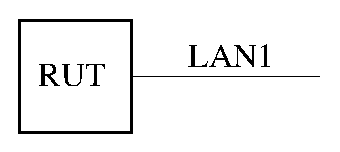
\includegraphics[scale=0.8]{figs/pim_test_6_1_single_bsr_election}
    \caption{Single BSR election test setup}
    \label{fig:single_bsr_election}
  \end{center}
\end{figure}

\para{Procedure:}
\begin{enumerate}

  \item Start the RUT.

  \item Check immediately the BSR status on the RUT. Initially the RUT should
        be the BSR in Pending state:

\begin{verbatim}
Xorp> show pim bootstrap
Active zones:
BSR              Pri LocalAddress     Pri State            Timeout
10.3.0.1           1 10.3.0.1           1 Pending               11
Configured zones:
BSR              Pri LocalAddress     Pri State            Timeout
10.3.0.1           1 10.3.0.1           1 Init                  -1
\end{verbatim}

  \item After \verb=BS_Timeout= ({\PimsmBSTimeout}), the RUT must become the
        elected BSR:

\begin{verbatim}
Xorp> show pim bootstrap
Active zones:
BSR              Pri LocalAddress     Pri State            Timeout
10.3.0.1           1 10.3.0.1           1 Elected               59
Configured zones:
BSR              Pri LocalAddress     Pri State            Timeout
10.3.0.1           1 10.3.0.1           1 Init                  -1
\end{verbatim}

\end{enumerate}


\para{Observable Results:}
TODO

\para{Possible Problems:}
The RUT might become the BSR earlier than \verb=BS_Timeout= ({\PimsmBSTimeout})
if the implementation uses a shorter timeout interval on startup (\eg
if it has tuned for fast start-up).

%%%%%%%%%%%%%%%%%%%%%%%%%%%%%%%%%%%%%%%%%%%
\newpage
\section{Single Router RP-Set}
\label{sec:bootstrap_mechanism:single_router_rpset}

\para{Purpose:}
Test if the Bootstrap-derived RP-Set works on a single router.

\para{References:}
\begin{itemize}

  \item draft-ietf-pim-sm-bsr-02 -- Section 3

\end{itemize}

\para{Discussion:}
A router that is both a candidate-BSR and a candidate-RP
must be able to include itself to the Cand-RP-Set.
The time to complete the election is
\verb=BS_Timeout= + up to (\verb=BS_Period= + \verb=C-RP-Adv-Period=) (\ie
$\leq$ ({\PimsmBSTimeout}) + ({\PimsmBSTimeout}) + ({\PimsmCRPAdvPeriod})).

\para{Test Setup:}
Connect the RUT according to Figure~\ref{fig:single_router_rp_set}.
Configure the RUT as a Cand-BSR and a Cand-RP.

\begin{figure}[htbp]
  \begin{center}
    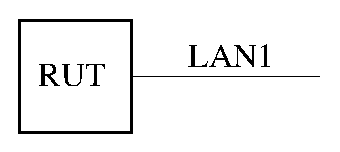
\includegraphics[scale=0.8]{figs/pim_test_6_2_single_router_rpset}
    \caption{Single router RP-Set test setup}
    \label{fig:single_router_rp_set}
  \end{center}
\end{figure}

\para{Procedure:}
\begin{enumerate}

  \item Start the RUT.

  \item Check immediately the RP-Set on the RUT. Initially the RUT should be
  empty:

\begin{verbatim}
Xorp> show pim rps
RP              Type      Pri Holdtime Timeout ActiveGroups GroupPrefix
\end{verbatim}

  \item After up to \verb=BS_Timeout= + \verb=BS_Period= +
        \verb=C-RP-Adv-Period=
        (\ie $\leq$ ({\PimsmBSTimeout}) + ({\PimsmBSTimeout}) +
        ({\PimsmCRPAdvPeriod})), the RUT must have a non-empty RP-Set with
        itself included in that set:

\begin{verbatim}
Xorp> show pim rps
RP              Type      Pri Holdtime Timeout ActiveGroups GroupPrefix
10.3.0.1        bootstrap 192       60      -1            0 224.0.0.0/4
\end{verbatim}

\end{enumerate}


\para{Observable Results:}
TODO

\para{Possible Problems:}
The RP-Set in the RUT might become non-empty much earlier than
\verb=BS_Timeout= + \verb=BS_Period= + \verb=C-RP-Adv-Period= (\ie $\leq$
({\PimsmBSTimeout}) + ({\PimsmBSTimeout}) + ({\PimsmCRPAdvPeriod}))
if the implementation uses shorter timeout intervals on startup (\eg
if it has tuned for fast start-up).

%%%%%%%%%%%%%%%%%%%%%%%%%%%%%%%%%%%%%%%%%%%
\newpage
\section{Bootstrap Timeout}

\para{Purpose:}
Test the Bootstrap timeout between two routers.

\para{References:}
\begin{itemize}
  \item draft-ietf-pim-sm-bsr-02 -- Section 3
\end{itemize}

\para{Discussion:}
If the elected BSR goes away, it should timeout in the
state of other routers. If it is gracefully shutdown, the BSR should send a
Bootstrap message with holdtime of 0, \ie the timeout should be almost
immediately.
If the BSR crashes, it should take up to \verb=BS_Timeout= ({\PimsmBSTimeout})
to timeout the state.

\para{Test Setup:}
Connect the RUT and TR1 according to Figure~\ref{fig:bootstrap_timeout}.
Configure TR1 as a Cand-BSR and a Cand-RP. Do not configure the RUT as a
Cand-BSR or a Cand-RP.

\begin{figure}[htbp]
  \begin{center}
    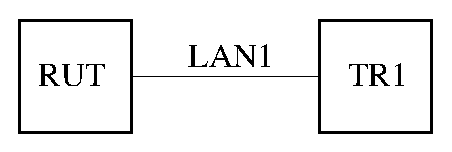
\includegraphics[scale=0.8]{figs/pim_test_6_3_bootstrap_timeout}
    \caption{Bootstrap timeout test setup}
    \label{fig:bootstrap_timeout}
  \end{center}
\end{figure}

\para{Procedure:}
\begin{enumerate}

  \item Start the RUT.

  \item Check that the RUT does not have any BSR or RP-related entries:

\begin{verbatim}
Xorp> show pim bootstrap
Active zones:
BSR              Pri LocalAddress     Pri State            Timeout
Configured zones:
BSR              Pri LocalAddress     Pri State            Timeout

Xorp> show pim rps
RP              Type      Pri Holdtime Timeout ActiveGroups GroupPrefix

Xorp> show pim join all
Group           Source          RP              Flags

\end{verbatim}

  \item Start TR1.

  \item After up to \verb=BS_Timeout= + \verb=BS_Period= +
        \verb=C-RP-Adv-Period=
        (\ie $\leq$ ({\PimsmBSTimeout}) + ({\PimsmBSTimeout}) +
        ({\PimsmCRPAdvPeriod})), the RUT must have a non-empty RP-Set
        with TR1 included in that set:

\begin{verbatim}
Xorp> show pim bootstrap
Active zones:
BSR              Pri LocalAddress     Pri State            Timeout
10.3.0.1           1 0.0.0.0            0 AcceptPreferred      122
Configured zones:
BSR              Pri LocalAddress     Pri State            Timeout

Xorp> show pim rps
RP              Type      Pri Holdtime Timeout ActiveGroups GroupPrefix
10.3.0.1        bootstrap 192       60      19            0 224.0.0.0/4

Xorp> show pim join all
Group           Source          RP              Flags
224.0.0.0       10.3.0.1        10.3.0.1        RP
    Upstream interface (S): UNKNOWN
    Upstream interface (RP): dc2
    Upstream state: NotJoined
    Register state:
    Join timer: -1
    Local include:            .............
    Local exclude:            .............
    Local include WC:         .............
    Local include SG:         .............
    Local exclude SG:         .............
    Joins RP:                 .............
    Joins WC:                 .............
    Joins SG:                 .............
    Prunes SG_RPT:            .............
    Join state:               .............
    Prune state:              .............
    Prune pending state:      .............
    I am assert winner state: .............
    I am assert loser state:  .............
    Assert winner WC:         .............
    Assert winner SG:         .............
    Assert lost WC:           .............
    Could assert SG:          .............
    I am DR:                  ....O........
    Immediate olist RP:       .............
    Immediate olist WC:       .............
    Immediate olist SG:       .............
    Inherited olist SG:       .............
    Inherited olist SG_RPT:   .............
    PIM include WC:           .............
\end{verbatim}

  \item Stop TR1.

  \item Wait until the BSR entry in the RUT timeout (up to \verb=BS_Period=
        ({\PimsmBSPeriod})). After that the RUT should show the BSR entry as
        expired, though it may still cache it in the scope zone entry.
        However, the RP-related entry might be deleted (though the spec
        allows caching them):

\begin{verbatim}
Xorp> show pim bootstrap
Active zones:
BSR              Pri LocalAddress     Pri State            Timeout SZTimeout
10.3.0.1           1 0.0.0.0            0 AcceptAny              0      1369
Configured zones:
BSR              Pri LocalAddress     Pri State            Timeout SZTimeout

Xorp> show pim rps
RP              Type      Pri Holdtime Timeout ActiveGroups GroupPrefix
Xorp> show pim join all
Group           Source          RP              Flags
\end{verbatim}

  \item After the Scope Zone in the RUT timeout, the RUT should not contain any
        scope zone entries:

\begin{verbatim}
Xorp> show pim bootstrap
Active zones:
BSR              Pri LocalAddress     Pri State            Timeout SZTimeout
Configured zones:
BSR              Pri LocalAddress     Pri State            Timeout SZTimeout
\end{verbatim}

\end{enumerate}


\para{Observable Results:}
TODO

\para{Possible Problems:}
TODO

%%%%%%%%%%%%%%%%%%%%%%%%%%%%%%%%%%%%%%%%%%%%%%%%%%%%%%%%%%%%%%%%%%%%%%%
\chapter{Multicast Routing Table}

\para{Scope:}
TODO

\para{Overview:}
TODO

%%%%%%%%%%%%%%%%%%%%%%%%%%%%%%%%%%%%%%%%%%%
\newpage
\section{Single Router Same-LAN Membership}

\para{Purpose:}
Test the same-LAN membership on a single router.

\para{References:}
\begin{itemize}
  \item draft-ietf-pim-sm-v2-new-05 -- Section 4.1.6
\end{itemize}

\para{Discussion:}
A router that has same-LAN group-specific or
source-group-specific member must be able to detect it and create the
appropriate MRE state in the MRT.

\para{Test Setup:}
Connect the RUT and Rx1 according to
Figure~\ref{fig:single_router_same_lan_membership}.
Configure the RUT as a Cand-BSR and a Cand-RP.

\begin{figure}[htbp]
  \begin{center}
    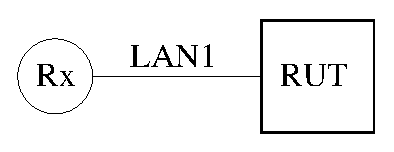
\includegraphics[scale=0.8]{figs/pim_test_7_1_single_router_samelan_membership}
    \caption{Single router Same-LAN membership test setup}
    \label{fig:single_router_same_lan_membership}
  \end{center}
\end{figure}

\para{Procedure:}

\subpara{Part A: Group-specific same-LAN membership.}

\begin{enumerate}

  \item Start the RUT.

  \item Wait until the RP-Set of the RUT becomes non-empty (\eg see
        \ref{sec:bootstrap_mechanism:single_router_rpset}).

  \item Test that the RUT has no local membership state:

\begin{verbatim}
Xorp> show pim join
Group           Source          RP              Flags
\end{verbatim}

  \item Start receiver Rx for group 224.0.1.20. For example:

\begin{verbatim}
root@xorp1[42] msend -i 10.2.0.1 -r 224.0.1.20/12345
\end{verbatim}

  \item Test that the RUT now has local membership for group 224.0.1.20:

\begin{verbatim}
Xorp> show pim join
Group           Source          RP              Flags
224.0.1.20      0.0.0.0         10.3.0.1        WC
    Upstream interface (S): UNKNOWN
    Upstream interface (RP): register_vif
    Upstream state: Joined
    Register state:
    Join timer: 57
    Local include:            ......O.......
    Local exclude:            ..............
    Local include WC:         ......O.......
    Local include SG:         ..............
    Local exclude SG:         ..............
    Joins RP:                 ..............
    Joins WC:                 ..............
    Joins SG:                 ..............
    Prunes SG_RPT:            ..............
    Join state:               ..............
    Prune state:              ..............
    Prune pending state:      ..............
    I am assert winner state: ..............
    I am assert loser state:  ..............
    Assert winner WC:         ..............
    Assert winner SG:         ..............
    Assert lost WC:           ..............
    Could assert SG:          ..............
    I am DR:                  .....OO.......
    Immediate olist RP:       ..............
    Immediate olist WC:       ......O.......
    Immediate olist SG:       ..............
    Inherited olist SG:       ..............
    Inherited olist SG_RPT:   ..............
    PIM include WC:           ......O.......
\end{verbatim}

  \item Stop receiver Rx

  \item Test that the RUT now has no local membership for group 224.0.1.20:

\begin{verbatim}
Xorp> show pim join
Group           Source          RP              Flags
\end{verbatim}

\end{enumerate}

\subpara{Part B: Source-group-specific same-LAN membership.}

\begin{enumerate}

  \item Start the RUT.

  \item Wait until the RP-Set of the RUT becomes non-empty (\eg see
        \ref{sec:bootstrap_mechanism:single_router_rpset}).

  \item Test that the RUT has no local membership state:

\begin{verbatim}
Xorp> show pim join
Group           Source          RP              Flags
\end{verbatim}

  \item TODO: Start receiver Rx for...

  \item TODO: Test that the RUT now has local membership for...

  \item Stop receiver Rx

  \item TODO: Test that the RUT now has no local membership for...

\begin{verbatim}
Xorp> show pim join
Group           Source          RP              Flags
\end{verbatim}

\end{enumerate}

\para{Observable Results:}
TODO

\para{Possible Problems:}
TODO

%%%%%%%%%%%%%%%%%%%%%%%%%%%%%%%%%%%%%%%%%%%
\newpage
\section{Template}

\para{Purpose:}
TODO

\para{References:}
\begin{itemize}
  \item draft-ietf-pim-sm-v2-new-05 -- Section TODO
\end{itemize}

\para{Discussion:}
TODO

\para{Test Setup:}
TODO

\para{Procedure:}
TODO

\para{Observable Results:}
TODO

\para{Possible Problems:}
TODO

%%%%%%%%%%%%%%%%%%%%%%%%%%%%%%%%%%%%%%%%%%%%%%%%%%%%%%%%%%%%%%%%%%%%%%%
%     BIBLIOGRAPHY
%%%%%%%%%%%%%%%%%%%%%%%%%%%%%%%%%%%%%%%%%%%%%%%%%%%%%%%%%%%%%%%%%%%%%%%

% \bibliography{pim_testsuite}
% \bibliographystyle{plain}

\end{document}

% \begin{figure}[htbp]
%   \begin{center}
%     \includegraphics[width=5.0in]{figs/pim_test_1_1_foo}
%     \caption{TODO}
%     \label{fig:TODO}
%   \end{center}
% \end{figure}
